\documentclass[twoside]{book}

% Packages required by doxygen
\usepackage{fixltx2e}
\usepackage{calc}
\usepackage{doxygen}
\usepackage[export]{adjustbox} % also loads graphicx
\usepackage{graphicx}
\usepackage[utf8]{inputenc}
\usepackage{makeidx}
\usepackage{multicol}
\usepackage{multirow}
\PassOptionsToPackage{warn}{textcomp}
\usepackage{textcomp}
\usepackage[nointegrals]{wasysym}
\usepackage[table]{xcolor}

% NLS support packages
\usepackage{polski}
\usepackage[T1]{fontenc}

% Font selection
\usepackage[T1]{fontenc}
\usepackage[scaled=.90]{helvet}
\usepackage{courier}
\usepackage{amssymb}
\usepackage{sectsty}
\renewcommand{\familydefault}{\sfdefault}
\allsectionsfont{%
  \fontseries{bc}\selectfont%
  \color{darkgray}%
}
\renewcommand{\DoxyLabelFont}{%
  \fontseries{bc}\selectfont%
  \color{darkgray}%
}
\newcommand{\+}{\discretionary{\mbox{\scriptsize$\hookleftarrow$}}{}{}}

% Page & text layout
\usepackage{geometry}
\geometry{%
  a4paper,%
  top=2.5cm,%
  bottom=2.5cm,%
  left=2.5cm,%
  right=2.5cm%
}
\tolerance=750
\hfuzz=15pt
\hbadness=750
\setlength{\emergencystretch}{15pt}
\setlength{\parindent}{0cm}
\setlength{\parskip}{3ex plus 2ex minus 2ex}
\makeatletter
\renewcommand{\paragraph}{%
  \@startsection{paragraph}{4}{0ex}{-1.0ex}{1.0ex}{%
    \normalfont\normalsize\bfseries\SS@parafont%
  }%
}
\renewcommand{\subparagraph}{%
  \@startsection{subparagraph}{5}{0ex}{-1.0ex}{1.0ex}{%
    \normalfont\normalsize\bfseries\SS@subparafont%
  }%
}
\makeatother

% Headers & footers
\usepackage{fancyhdr}
\pagestyle{fancyplain}
\fancyhead[LE]{\fancyplain{}{\bfseries\thepage}}
\fancyhead[CE]{\fancyplain{}{}}
\fancyhead[RE]{\fancyplain{}{\bfseries\leftmark}}
\fancyhead[LO]{\fancyplain{}{\bfseries\rightmark}}
\fancyhead[CO]{\fancyplain{}{}}
\fancyhead[RO]{\fancyplain{}{\bfseries\thepage}}
\fancyfoot[LE]{\fancyplain{}{}}
\fancyfoot[CE]{\fancyplain{}{}}
\fancyfoot[RE]{\fancyplain{}{\bfseries\scriptsize Wygenerowano przez Doxygen }}
\fancyfoot[LO]{\fancyplain{}{\bfseries\scriptsize Wygenerowano przez Doxygen }}
\fancyfoot[CO]{\fancyplain{}{}}
\fancyfoot[RO]{\fancyplain{}{}}
\renewcommand{\footrulewidth}{0.4pt}
\renewcommand{\chaptermark}[1]{%
  \markboth{#1}{}%
}
\renewcommand{\sectionmark}[1]{%
  \markright{\thesection\ #1}%
}

% Indices & bibliography
\usepackage{natbib}
\usepackage[titles]{tocloft}
\setcounter{tocdepth}{3}
\setcounter{secnumdepth}{5}
\makeindex

% Hyperlinks (required, but should be loaded last)
\usepackage{ifpdf}
\ifpdf
  \usepackage[pdftex,pagebackref=true]{hyperref}
\else
  \usepackage[ps2pdf,pagebackref=true]{hyperref}
\fi
\hypersetup{%
  colorlinks=true,%
  linkcolor=blue,%
  citecolor=blue,%
  unicode%
}

% Custom commands
\newcommand{\clearemptydoublepage}{%
  \newpage{\pagestyle{empty}\cleardoublepage}%
}

\usepackage{caption}
\captionsetup{labelsep=space,justification=centering,font={bf},singlelinecheck=off,skip=4pt,position=top}

%===== C O N T E N T S =====

\begin{document}

% Titlepage & ToC
\hypersetup{pageanchor=false,
             bookmarksnumbered=true,
             pdfencoding=unicode
            }
\pagenumbering{alph}
\begin{titlepage}
\vspace*{7cm}
\begin{center}%
{\Large Lampki\+App }\\
\vspace*{1cm}
{\large Wygenerowano przez Doxygen 1.8.14}\\
\end{center}
\end{titlepage}
\clearemptydoublepage
\pagenumbering{roman}
\tableofcontents
\clearemptydoublepage
\pagenumbering{arabic}
\hypersetup{pageanchor=true}

%--- Begin generated contents ---
\chapter{Indeks hierarchiczny}
\section{Hierarchia klas}
Ta lista dziedziczenia posortowana jest z grubsza, choć nie całkowicie, alfabetycznie\+:\begin{DoxyCompactList}
\item \contentsline{section}{A\+Color\+Model}{\pageref{class_a_color_model}}{}
\begin{DoxyCompactList}
\item \contentsline{section}{H\+S\+V\+Color\+Model}{\pageref{class_h_s_v_color_model}}{}
\item \contentsline{section}{R\+G\+B\+Color\+Model}{\pageref{class_r_g_b_color_model}}{}
\end{DoxyCompactList}
\item \contentsline{section}{J\+S\+O\+N\+Helper}{\pageref{class_j_s_o_n_helper}}{}
\item Q\+Object\begin{DoxyCompactList}
\item \contentsline{section}{Color\+View\+Model}{\pageref{class_color_view_model}}{}
\item \contentsline{section}{Gradient\+View\+Model}{\pageref{class_gradient_view_model}}{}
\item \contentsline{section}{Rest\+Helper}{\pageref{class_rest_helper}}{}
\item \contentsline{section}{settings\+View\+Model}{\pageref{classsettings_view_model}}{}
\end{DoxyCompactList}
\end{DoxyCompactList}

\chapter{Indeks klas}
\section{Lista klas}
Tutaj znajdują się klasy, struktury, unie i interfejsy wraz z ich krótkimi opisami\+:\begin{DoxyCompactList}
\item\contentsline{section}{\mbox{\hyperlink{class_a_color_model}{A\+Color\+Model}} \\*The \mbox{\hyperlink{class_a_color_model}{A\+Color\+Model}} class Klasa abstrakcyjna stanowiąca interfejs dla klas modeli kolorów w przestrzeniach R\+GB i H\+SV }{\pageref{class_a_color_model}}{}
\item\contentsline{section}{\mbox{\hyperlink{class_color_view_model}{Color\+View\+Model}} \\*The \mbox{\hyperlink{class_color_view_model}{Color\+View\+Model}} class Klasa służy do komunikacji między modelami \mbox{\hyperlink{class_h_s_v_color_model}{H\+S\+V\+Color\+Model}} oraz \mbox{\hyperlink{class_r_g_b_color_model}{R\+G\+B\+Color\+Model}} a interfejsem użytkownika }{\pageref{class_color_view_model}}{}
\item\contentsline{section}{\mbox{\hyperlink{class_gradient_view_model}{Gradient\+View\+Model}} \\*The \mbox{\hyperlink{class_gradient_view_model}{Gradient\+View\+Model}} class Klasa pozwala na obsługę tworzenia gradientu dwukolorowego }{\pageref{class_gradient_view_model}}{}
\item\contentsline{section}{\mbox{\hyperlink{class_h_s_v_color_model}{H\+S\+V\+Color\+Model}} \\*The \mbox{\hyperlink{class_h_s_v_color_model}{H\+S\+V\+Color\+Model}} class Klasa dziedziczy po abstrakcyjnej klasie \mbox{\hyperlink{class_a_color_model}{A\+Color\+Model}}. Odpowiada za przetwarzanie danych dotyczacych koloru w przestrzeni barw H\+SV }{\pageref{class_h_s_v_color_model}}{}
\item\contentsline{section}{\mbox{\hyperlink{class_j_s_o_n_helper}{J\+S\+O\+N\+Helper}} \\*The \mbox{\hyperlink{class_j_s_o_n_helper}{J\+S\+O\+N\+Helper}} class Klasa przygotowuje dane do przesłania poprzez zapisanie danych na temat ustawionych kolorów diod w Java\+Script Object Notation. Klasa jest zgodna z wzorcem Singleton }{\pageref{class_j_s_o_n_helper}}{}
\item\contentsline{section}{\mbox{\hyperlink{class_rest_helper}{Rest\+Helper}} \\*The \mbox{\hyperlink{class_rest_helper}{Rest\+Helper}} class Klasa obsługuje wymianę danych pomiędzy aplikacją a A\+PI urządzenia Raspberry\+Pi. Klasa zgodna z wzorcem Singleton }{\pageref{class_rest_helper}}{}
\item\contentsline{section}{\mbox{\hyperlink{class_r_g_b_color_model}{R\+G\+B\+Color\+Model}} \\*The \mbox{\hyperlink{class_r_g_b_color_model}{R\+G\+B\+Color\+Model}} class Klasa dziedziczy po abstrakcyjnej klasie \mbox{\hyperlink{class_a_color_model}{A\+Color\+Model}}. Odpowiada za przetwarzanie danych dotyczacych koloru w przestrzeni barw R\+GB }{\pageref{class_r_g_b_color_model}}{}
\item\contentsline{section}{\mbox{\hyperlink{classsettings_view_model}{settings\+View\+Model}} \\*Klasa obsługuje komunikację między Rest\+Helperem a UI -\/ pozwala na modyfikację przez użytkownika ustawień połączenia z urządzeniem Raspberry PI }{\pageref{classsettings_view_model}}{}
\end{DoxyCompactList}

\chapter{Dokumentacja klas}
\hypertarget{class_a_color_model}{}\section{Dokumentacja klasy A\+Color\+Model}
\label{class_a_color_model}\index{A\+Color\+Model@{A\+Color\+Model}}


The \mbox{\hyperlink{class_a_color_model}{A\+Color\+Model}} class Klasa abstrakcyjna stanowiąca interfejs dla klas modeli kolorów w przestrzeniach R\+GB i H\+SV.  




{\ttfamily \#include $<$acolormodel.\+h$>$}

Diagram dziedziczenia dla A\+Color\+Model\begin{figure}[H]
\begin{center}
\leavevmode
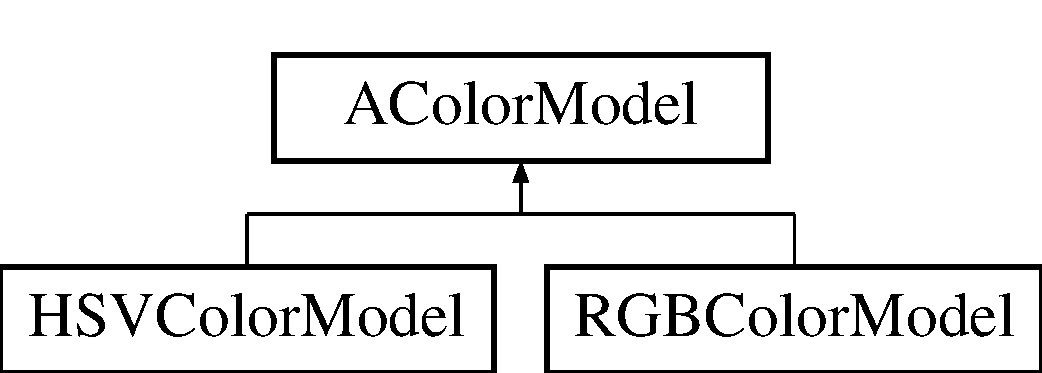
\includegraphics[height=2.000000cm]{class_a_color_model}
\end{center}
\end{figure}
\subsection*{Metody publiczne}
\begin{DoxyCompactItemize}
\item 
\mbox{\Hypertarget{class_a_color_model_a4470865f3afc2f31e710d9a59d03977a}\label{class_a_color_model_a4470865f3afc2f31e710d9a59d03977a}} 
virtual std\+::unique\+\_\+ptr$<$ \mbox{\hyperlink{class_a_color_model}{A\+Color\+Model}} $>$ {\bfseries As\+R\+GB} ()=0
\item 
\mbox{\Hypertarget{class_a_color_model_a12340b3af356d03303b15717ca4ba042}\label{class_a_color_model_a12340b3af356d03303b15717ca4ba042}} 
virtual std\+::unique\+\_\+ptr$<$ \mbox{\hyperlink{class_a_color_model}{A\+Color\+Model}} $>$ {\bfseries As\+H\+SV} ()=0
\item 
\mbox{\Hypertarget{class_a_color_model_a64682636f42f22b9c90bc0f41d6b6993}\label{class_a_color_model_a64682636f42f22b9c90bc0f41d6b6993}} 
virtual Q\+String {\bfseries As\+Hex} ()=0
\item 
\mbox{\Hypertarget{class_a_color_model_a8919f286412465faaa8d17ed4251889f}\label{class_a_color_model_a8919f286412465faaa8d17ed4251889f}} 
virtual int {\bfseries Get\+RH} ()=0
\item 
\mbox{\Hypertarget{class_a_color_model_a05e7b42a530a9856636c87111ee4c2ee}\label{class_a_color_model_a05e7b42a530a9856636c87111ee4c2ee}} 
virtual int {\bfseries Get\+GS} ()=0
\item 
\mbox{\Hypertarget{class_a_color_model_a9ea2fa3db7783570f6ac38c75206e979}\label{class_a_color_model_a9ea2fa3db7783570f6ac38c75206e979}} 
virtual int {\bfseries Get\+BV} ()=0
\item 
\mbox{\Hypertarget{class_a_color_model_aa6eb3eb0741790d4a624875cb3d18d6f}\label{class_a_color_model_aa6eb3eb0741790d4a624875cb3d18d6f}} 
virtual void {\bfseries Set\+RH} (int rh)=0
\item 
\mbox{\Hypertarget{class_a_color_model_a009adc0bb0e2586c0b111fdbf0cb58d1}\label{class_a_color_model_a009adc0bb0e2586c0b111fdbf0cb58d1}} 
virtual void {\bfseries Set\+GS} (int gs)=0
\item 
\mbox{\Hypertarget{class_a_color_model_a645fa27531dc1a37136bc9dd5035104f}\label{class_a_color_model_a645fa27531dc1a37136bc9dd5035104f}} 
virtual void {\bfseries Set\+BV} (int bv)=0
\end{DoxyCompactItemize}


\subsection{Opis szczegółowy}
The \mbox{\hyperlink{class_a_color_model}{A\+Color\+Model}} class Klasa abstrakcyjna stanowiąca interfejs dla klas modeli kolorów w przestrzeniach R\+GB i H\+SV. 

Dokumentacja dla tej klasy została wygenerowana z pliku\+:\begin{DoxyCompactItemize}
\item 
C\+:/\+Users/amy1/\+Source/\+Qt/\+Lampki\+App/\+Models/acolormodel.\+h\end{DoxyCompactItemize}

\hypertarget{class_color_view_model}{}\section{Dokumentacja klasy Color\+View\+Model}
\label{class_color_view_model}\index{Color\+View\+Model@{Color\+View\+Model}}


The \mbox{\hyperlink{class_color_view_model}{Color\+View\+Model}} class Klasa służy do komunikacji między modelami \mbox{\hyperlink{class_h_s_v_color_model}{H\+S\+V\+Color\+Model}} oraz \mbox{\hyperlink{class_r_g_b_color_model}{R\+G\+B\+Color\+Model}} a interfejsem użytkownika.  




{\ttfamily \#include $<$colorviewmodel.\+h$>$}

Diagram dziedziczenia dla Color\+View\+Model\begin{figure}[H]
\begin{center}
\leavevmode
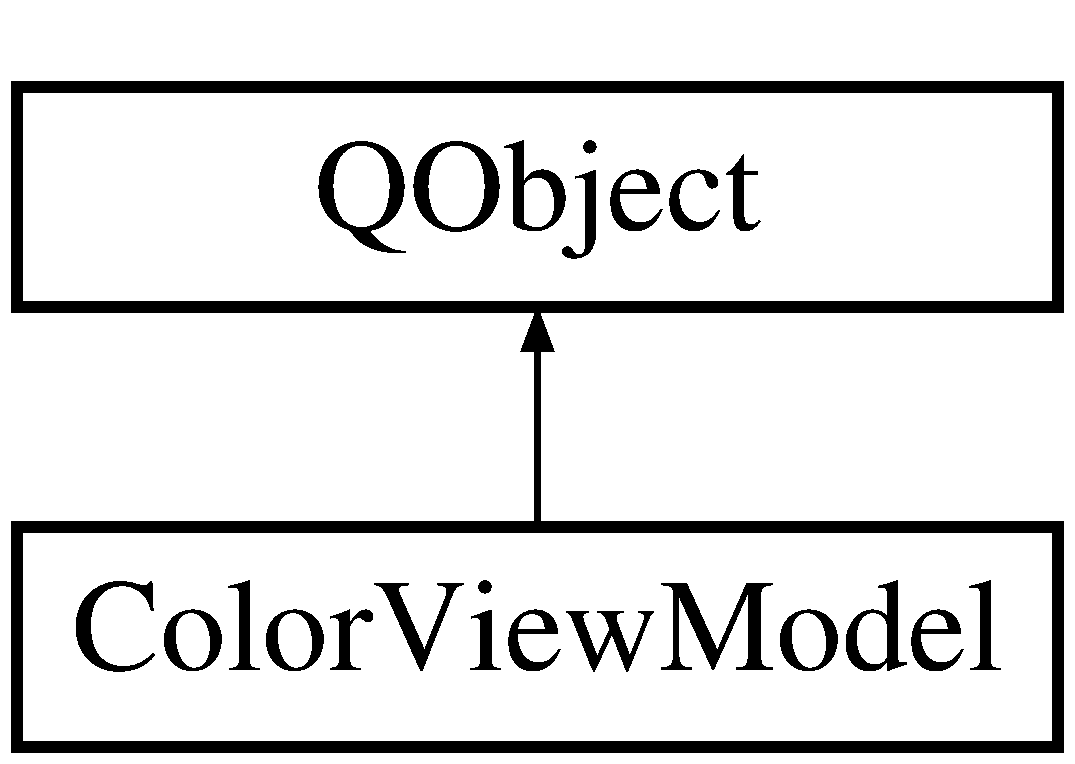
\includegraphics[height=2.000000cm]{class_color_view_model}
\end{center}
\end{figure}
\subsection*{Sloty publiczne}
\begin{DoxyCompactItemize}
\item 
void \mbox{\hyperlink{class_color_view_model_a0e3aa4fdb5fd3f05d3bd5c82ee571c91}{Set\+RH}} (int rh)
\begin{DoxyCompactList}\small\item\em Set\+RH Modyfikuje właściwość RH. \end{DoxyCompactList}\item 
void \mbox{\hyperlink{class_color_view_model_a7ef1ac038793902b460f5b65a66ba063}{Set\+GS}} (int gs)
\begin{DoxyCompactList}\small\item\em Set\+GS Modyfikuje właściwość GS. \end{DoxyCompactList}\item 
void \mbox{\hyperlink{class_color_view_model_a07fbf050b15842e8e68c32c44ef9c6dd}{Set\+BV}} (int bv)
\begin{DoxyCompactList}\small\item\em Set\+BV Modyfikuje właściwość BV. \end{DoxyCompactList}\item 
void \mbox{\hyperlink{class_color_view_model_a51b5ff8b09631334b01ad95e0559452f}{set\+Selected\+Type}} (int selection)
\begin{DoxyCompactList}\small\item\em set\+Selected\+Type Modyfikuje właściwość Selected\+Type, wywołuje konwersję między przestrzeniami H\+SV i R\+GB \end{DoxyCompactList}\item 
void \mbox{\hyperlink{class_color_view_model_ae5d39c213d8ef75346766d006e55e142}{Set\+Hex}} (Q\+String hex)
\begin{DoxyCompactList}\small\item\em Set\+Hex Modyfikuje właściwość Hex. \end{DoxyCompactList}\end{DoxyCompactItemize}
\subsection*{Sygnały}
\begin{DoxyCompactItemize}
\item 
void \mbox{\hyperlink{class_color_view_model_ae82220bcc3ce7136ae025d8ba84c1ef5}{R\+H\+Changed}} (int arg)
\begin{DoxyCompactList}\small\item\em R\+H\+Changed Informuje o zmianie właściwości RH. \end{DoxyCompactList}\item 
void \mbox{\hyperlink{class_color_view_model_ab36d827240046bae55a0a7e18b50fcc3}{G\+S\+Changed}} (int arg)
\begin{DoxyCompactList}\small\item\em G\+S\+Changed Informuje o zmianie właściwości GS. \end{DoxyCompactList}\item 
void \mbox{\hyperlink{class_color_view_model_a242d8b688b15906ff79ab0a01f5877fc}{B\+V\+Changed}} (int arg)
\begin{DoxyCompactList}\small\item\em B\+V\+Changed Informuje o zmianie właściwości BV. \end{DoxyCompactList}\item 
void \mbox{\hyperlink{class_color_view_model_a40e736b58e641078c43dcf146a4b53bd}{selected\+Type\+Changed}} (int arg)
\begin{DoxyCompactList}\small\item\em selected\+Type\+Changed Informuje o zmianie wybranej przestrzeni barw \end{DoxyCompactList}\item 
void \mbox{\hyperlink{class_color_view_model_aff6ce1151bebe9048a61b99742ad6492}{hex\+Changed}} (Q\+String arg)
\begin{DoxyCompactList}\small\item\em hex\+Changed Informuje o zmianie kodu szesnastkowego koloru \end{DoxyCompactList}\end{DoxyCompactItemize}
\subsection*{Metody publiczne}
\begin{DoxyCompactItemize}
\item 
\mbox{\Hypertarget{class_color_view_model_ac76a50243490a747fecb1c89bc2dd1be}\label{class_color_view_model_ac76a50243490a747fecb1c89bc2dd1be}} 
{\bfseries Color\+View\+Model} (Q\+Object $\ast$parent=nullptr)
\item 
int \mbox{\hyperlink{class_color_view_model_a39724a979609cf96d76a905f313b18c6}{Get\+RH}} ()
\begin{DoxyCompactList}\small\item\em Get\+RH Zwraca wartość składowej Hue lub Red -\/ w zależności od kontekstu. \end{DoxyCompactList}\item 
int \mbox{\hyperlink{class_color_view_model_a82022dc5932e3c485e7f387b47251587}{Get\+GS}} ()
\begin{DoxyCompactList}\small\item\em Get\+GS Zwraca wartość składowej Saturation lub Green -\/ w zależności od kontekstu. \end{DoxyCompactList}\item 
int \mbox{\hyperlink{class_color_view_model_ab2ee304b2a6b4ff3945fe926acd575b4}{Get\+BV}} ()
\begin{DoxyCompactList}\small\item\em Get\+BV Zwraca wartość składowej Value lub Blue -\/ w zależności od kontekstu. \end{DoxyCompactList}\item 
int \mbox{\hyperlink{class_color_view_model_a02a51cd04a027d369275cb29229c44c7}{get\+Selected\+Type}} ()
\begin{DoxyCompactList}\small\item\em get\+Selected\+Type Zwraca informację o wybranej przestrzeni barw \end{DoxyCompactList}\item 
Q\+String \mbox{\hyperlink{class_color_view_model_a8288300fcaa560f71974038e0bc191ea}{Get\+Hex}} ()
\begin{DoxyCompactList}\small\item\em Get\+Hex. \end{DoxyCompactList}\item 
\mbox{\Hypertarget{class_color_view_model_a86906d53218bb80ef563040cb5e7ec30}\label{class_color_view_model_a86906d53218bb80ef563040cb5e7ec30}} 
Q\+\_\+\+I\+N\+V\+O\+K\+A\+B\+LE void \mbox{\hyperlink{class_color_view_model_a86906d53218bb80ef563040cb5e7ec30}{Send\+Unicolor}} ()
\begin{DoxyCompactList}\small\item\em Metoda wysyła dane na temat koloru do urządzenia. \end{DoxyCompactList}\end{DoxyCompactItemize}
\subsection*{Właściwości}
\begin{DoxyCompactItemize}
\item 
\mbox{\Hypertarget{class_color_view_model_ae0f5138a9621f84b1ded3ecff66d7762}\label{class_color_view_model_ae0f5138a9621f84b1ded3ecff66d7762}} 
int {\bfseries RH}
\item 
\mbox{\Hypertarget{class_color_view_model_a01554860f6ce1c2cc9be53085c6be31f}\label{class_color_view_model_a01554860f6ce1c2cc9be53085c6be31f}} 
int {\bfseries GS}
\item 
\mbox{\Hypertarget{class_color_view_model_ab56668fbfd75bd38ba255b0d7bf209e3}\label{class_color_view_model_ab56668fbfd75bd38ba255b0d7bf209e3}} 
int {\bfseries BV}
\item 
\mbox{\Hypertarget{class_color_view_model_ad9b6fd8d70e82197261dde9e25f53373}\label{class_color_view_model_ad9b6fd8d70e82197261dde9e25f53373}} 
int {\bfseries Selected\+Type}
\item 
\mbox{\Hypertarget{class_color_view_model_a5f3c225efc04ea48dd0be3133da6c660}\label{class_color_view_model_a5f3c225efc04ea48dd0be3133da6c660}} 
Q\+String {\bfseries Hex}
\end{DoxyCompactItemize}


\subsection{Opis szczegółowy}
The \mbox{\hyperlink{class_color_view_model}{Color\+View\+Model}} class Klasa służy do komunikacji między modelami \mbox{\hyperlink{class_h_s_v_color_model}{H\+S\+V\+Color\+Model}} oraz \mbox{\hyperlink{class_r_g_b_color_model}{R\+G\+B\+Color\+Model}} a interfejsem użytkownika. 

\subsection{Dokumentacja funkcji składowych}
\mbox{\Hypertarget{class_color_view_model_a242d8b688b15906ff79ab0a01f5877fc}\label{class_color_view_model_a242d8b688b15906ff79ab0a01f5877fc}} 
\index{Color\+View\+Model@{Color\+View\+Model}!B\+V\+Changed@{B\+V\+Changed}}
\index{B\+V\+Changed@{B\+V\+Changed}!Color\+View\+Model@{Color\+View\+Model}}
\subsubsection{\texorpdfstring{B\+V\+Changed}{BVChanged}}
{\footnotesize\ttfamily void Color\+View\+Model\+::\+B\+V\+Changed (\begin{DoxyParamCaption}\item[{int}]{arg }\end{DoxyParamCaption})\hspace{0.3cm}{\ttfamily [signal]}}



B\+V\+Changed Informuje o zmianie właściwości BV. 


\begin{DoxyParams}{Parametry}
{\em arg} & wartość liczbowa składowej Blue lub Value \\
\hline
\end{DoxyParams}
\mbox{\Hypertarget{class_color_view_model_ab2ee304b2a6b4ff3945fe926acd575b4}\label{class_color_view_model_ab2ee304b2a6b4ff3945fe926acd575b4}} 
\index{Color\+View\+Model@{Color\+View\+Model}!Get\+BV@{Get\+BV}}
\index{Get\+BV@{Get\+BV}!Color\+View\+Model@{Color\+View\+Model}}
\subsubsection{\texorpdfstring{Get\+B\+V()}{GetBV()}}
{\footnotesize\ttfamily int Color\+View\+Model\+::\+Get\+BV (\begin{DoxyParamCaption}{ }\end{DoxyParamCaption})}



Get\+BV Zwraca wartość składowej Value lub Blue -\/ w zależności od kontekstu. 

\begin{DoxyReturn}{Zwraca}
wartość liczbowa składowej Value lub Blue 
\end{DoxyReturn}
\mbox{\Hypertarget{class_color_view_model_a82022dc5932e3c485e7f387b47251587}\label{class_color_view_model_a82022dc5932e3c485e7f387b47251587}} 
\index{Color\+View\+Model@{Color\+View\+Model}!Get\+GS@{Get\+GS}}
\index{Get\+GS@{Get\+GS}!Color\+View\+Model@{Color\+View\+Model}}
\subsubsection{\texorpdfstring{Get\+G\+S()}{GetGS()}}
{\footnotesize\ttfamily int Color\+View\+Model\+::\+Get\+GS (\begin{DoxyParamCaption}{ }\end{DoxyParamCaption})}



Get\+GS Zwraca wartość składowej Saturation lub Green -\/ w zależności od kontekstu. 

\begin{DoxyReturn}{Zwraca}
wartość liczbowa składowej Saturation lub Green 
\end{DoxyReturn}
\mbox{\Hypertarget{class_color_view_model_a8288300fcaa560f71974038e0bc191ea}\label{class_color_view_model_a8288300fcaa560f71974038e0bc191ea}} 
\index{Color\+View\+Model@{Color\+View\+Model}!Get\+Hex@{Get\+Hex}}
\index{Get\+Hex@{Get\+Hex}!Color\+View\+Model@{Color\+View\+Model}}
\subsubsection{\texorpdfstring{Get\+Hex()}{GetHex()}}
{\footnotesize\ttfamily Q\+String Color\+View\+Model\+::\+Get\+Hex (\begin{DoxyParamCaption}{ }\end{DoxyParamCaption})}



Get\+Hex. 

\begin{DoxyReturn}{Zwraca}
kod szesnastkowy wybranego koloru 
\end{DoxyReturn}
\mbox{\Hypertarget{class_color_view_model_a39724a979609cf96d76a905f313b18c6}\label{class_color_view_model_a39724a979609cf96d76a905f313b18c6}} 
\index{Color\+View\+Model@{Color\+View\+Model}!Get\+RH@{Get\+RH}}
\index{Get\+RH@{Get\+RH}!Color\+View\+Model@{Color\+View\+Model}}
\subsubsection{\texorpdfstring{Get\+R\+H()}{GetRH()}}
{\footnotesize\ttfamily int Color\+View\+Model\+::\+Get\+RH (\begin{DoxyParamCaption}{ }\end{DoxyParamCaption})}



Get\+RH Zwraca wartość składowej Hue lub Red -\/ w zależności od kontekstu. 

\begin{DoxyReturn}{Zwraca}
wartość liczbowa składowej Hue lub Red 
\end{DoxyReturn}
\mbox{\Hypertarget{class_color_view_model_a02a51cd04a027d369275cb29229c44c7}\label{class_color_view_model_a02a51cd04a027d369275cb29229c44c7}} 
\index{Color\+View\+Model@{Color\+View\+Model}!get\+Selected\+Type@{get\+Selected\+Type}}
\index{get\+Selected\+Type@{get\+Selected\+Type}!Color\+View\+Model@{Color\+View\+Model}}
\subsubsection{\texorpdfstring{get\+Selected\+Type()}{getSelectedType()}}
{\footnotesize\ttfamily int Color\+View\+Model\+::get\+Selected\+Type (\begin{DoxyParamCaption}{ }\end{DoxyParamCaption})}



get\+Selected\+Type Zwraca informację o wybranej przestrzeni barw 

\begin{DoxyReturn}{Zwraca}
wartość liczbowa indeksu wybranego elementu w rozwijanej liście 
\end{DoxyReturn}
\mbox{\Hypertarget{class_color_view_model_ab36d827240046bae55a0a7e18b50fcc3}\label{class_color_view_model_ab36d827240046bae55a0a7e18b50fcc3}} 
\index{Color\+View\+Model@{Color\+View\+Model}!G\+S\+Changed@{G\+S\+Changed}}
\index{G\+S\+Changed@{G\+S\+Changed}!Color\+View\+Model@{Color\+View\+Model}}
\subsubsection{\texorpdfstring{G\+S\+Changed}{GSChanged}}
{\footnotesize\ttfamily void Color\+View\+Model\+::\+G\+S\+Changed (\begin{DoxyParamCaption}\item[{int}]{arg }\end{DoxyParamCaption})\hspace{0.3cm}{\ttfamily [signal]}}



G\+S\+Changed Informuje o zmianie właściwości GS. 


\begin{DoxyParams}{Parametry}
{\em arg} & wartość liczbowa składowej Green lub Saturation \\
\hline
\end{DoxyParams}
\mbox{\Hypertarget{class_color_view_model_aff6ce1151bebe9048a61b99742ad6492}\label{class_color_view_model_aff6ce1151bebe9048a61b99742ad6492}} 
\index{Color\+View\+Model@{Color\+View\+Model}!hex\+Changed@{hex\+Changed}}
\index{hex\+Changed@{hex\+Changed}!Color\+View\+Model@{Color\+View\+Model}}
\subsubsection{\texorpdfstring{hex\+Changed}{hexChanged}}
{\footnotesize\ttfamily void Color\+View\+Model\+::hex\+Changed (\begin{DoxyParamCaption}\item[{Q\+String}]{arg }\end{DoxyParamCaption})\hspace{0.3cm}{\ttfamily [signal]}}



hex\+Changed Informuje o zmianie kodu szesnastkowego koloru 


\begin{DoxyParams}{Parametry}
{\em arg} & łańcuch znaków z kodem szesnastkowym koloru \\
\hline
\end{DoxyParams}
\mbox{\Hypertarget{class_color_view_model_ae82220bcc3ce7136ae025d8ba84c1ef5}\label{class_color_view_model_ae82220bcc3ce7136ae025d8ba84c1ef5}} 
\index{Color\+View\+Model@{Color\+View\+Model}!R\+H\+Changed@{R\+H\+Changed}}
\index{R\+H\+Changed@{R\+H\+Changed}!Color\+View\+Model@{Color\+View\+Model}}
\subsubsection{\texorpdfstring{R\+H\+Changed}{RHChanged}}
{\footnotesize\ttfamily void Color\+View\+Model\+::\+R\+H\+Changed (\begin{DoxyParamCaption}\item[{int}]{arg }\end{DoxyParamCaption})\hspace{0.3cm}{\ttfamily [signal]}}



R\+H\+Changed Informuje o zmianie właściwości RH. 


\begin{DoxyParams}{Parametry}
{\em arg} & wartość liczbowa składowej Red lub Hue \\
\hline
\end{DoxyParams}
\mbox{\Hypertarget{class_color_view_model_a40e736b58e641078c43dcf146a4b53bd}\label{class_color_view_model_a40e736b58e641078c43dcf146a4b53bd}} 
\index{Color\+View\+Model@{Color\+View\+Model}!selected\+Type\+Changed@{selected\+Type\+Changed}}
\index{selected\+Type\+Changed@{selected\+Type\+Changed}!Color\+View\+Model@{Color\+View\+Model}}
\subsubsection{\texorpdfstring{selected\+Type\+Changed}{selectedTypeChanged}}
{\footnotesize\ttfamily void Color\+View\+Model\+::selected\+Type\+Changed (\begin{DoxyParamCaption}\item[{int}]{arg }\end{DoxyParamCaption})\hspace{0.3cm}{\ttfamily [signal]}}



selected\+Type\+Changed Informuje o zmianie wybranej przestrzeni barw 


\begin{DoxyParams}{Parametry}
{\em arg} & numer indeksu odpowiadającego wybranej przestrzeni barw \\
\hline
\end{DoxyParams}
\mbox{\Hypertarget{class_color_view_model_a07fbf050b15842e8e68c32c44ef9c6dd}\label{class_color_view_model_a07fbf050b15842e8e68c32c44ef9c6dd}} 
\index{Color\+View\+Model@{Color\+View\+Model}!Set\+BV@{Set\+BV}}
\index{Set\+BV@{Set\+BV}!Color\+View\+Model@{Color\+View\+Model}}
\subsubsection{\texorpdfstring{Set\+BV}{SetBV}}
{\footnotesize\ttfamily void Color\+View\+Model\+::\+Set\+BV (\begin{DoxyParamCaption}\item[{int}]{bv }\end{DoxyParamCaption})\hspace{0.3cm}{\ttfamily [slot]}}



Set\+BV Modyfikuje właściwość BV. 


\begin{DoxyParams}{Parametry}
{\em bv} & wartość przypisywana właściwości BV \\
\hline
\end{DoxyParams}
\mbox{\Hypertarget{class_color_view_model_a7ef1ac038793902b460f5b65a66ba063}\label{class_color_view_model_a7ef1ac038793902b460f5b65a66ba063}} 
\index{Color\+View\+Model@{Color\+View\+Model}!Set\+GS@{Set\+GS}}
\index{Set\+GS@{Set\+GS}!Color\+View\+Model@{Color\+View\+Model}}
\subsubsection{\texorpdfstring{Set\+GS}{SetGS}}
{\footnotesize\ttfamily void Color\+View\+Model\+::\+Set\+GS (\begin{DoxyParamCaption}\item[{int}]{gs }\end{DoxyParamCaption})\hspace{0.3cm}{\ttfamily [slot]}}



Set\+GS Modyfikuje właściwość GS. 


\begin{DoxyParams}{Parametry}
{\em gs} & wartość przypisywana właściwości GS \\
\hline
\end{DoxyParams}
\mbox{\Hypertarget{class_color_view_model_ae5d39c213d8ef75346766d006e55e142}\label{class_color_view_model_ae5d39c213d8ef75346766d006e55e142}} 
\index{Color\+View\+Model@{Color\+View\+Model}!Set\+Hex@{Set\+Hex}}
\index{Set\+Hex@{Set\+Hex}!Color\+View\+Model@{Color\+View\+Model}}
\subsubsection{\texorpdfstring{Set\+Hex}{SetHex}}
{\footnotesize\ttfamily void Color\+View\+Model\+::\+Set\+Hex (\begin{DoxyParamCaption}\item[{Q\+String}]{hex }\end{DoxyParamCaption})\hspace{0.3cm}{\ttfamily [slot]}}



Set\+Hex Modyfikuje właściwość Hex. 


\begin{DoxyParams}{Parametry}
{\em hex} & kod szesnastkowy koloru przypisywany właściwości Hex \\
\hline
\end{DoxyParams}
\mbox{\Hypertarget{class_color_view_model_a0e3aa4fdb5fd3f05d3bd5c82ee571c91}\label{class_color_view_model_a0e3aa4fdb5fd3f05d3bd5c82ee571c91}} 
\index{Color\+View\+Model@{Color\+View\+Model}!Set\+RH@{Set\+RH}}
\index{Set\+RH@{Set\+RH}!Color\+View\+Model@{Color\+View\+Model}}
\subsubsection{\texorpdfstring{Set\+RH}{SetRH}}
{\footnotesize\ttfamily void Color\+View\+Model\+::\+Set\+RH (\begin{DoxyParamCaption}\item[{int}]{rh }\end{DoxyParamCaption})\hspace{0.3cm}{\ttfamily [slot]}}



Set\+RH Modyfikuje właściwość RH. 


\begin{DoxyParams}{Parametry}
{\em rh} & wartość przypisywana właściwości RH \\
\hline
\end{DoxyParams}
\mbox{\Hypertarget{class_color_view_model_a51b5ff8b09631334b01ad95e0559452f}\label{class_color_view_model_a51b5ff8b09631334b01ad95e0559452f}} 
\index{Color\+View\+Model@{Color\+View\+Model}!set\+Selected\+Type@{set\+Selected\+Type}}
\index{set\+Selected\+Type@{set\+Selected\+Type}!Color\+View\+Model@{Color\+View\+Model}}
\subsubsection{\texorpdfstring{set\+Selected\+Type}{setSelectedType}}
{\footnotesize\ttfamily void Color\+View\+Model\+::set\+Selected\+Type (\begin{DoxyParamCaption}\item[{int}]{selection }\end{DoxyParamCaption})\hspace{0.3cm}{\ttfamily [slot]}}



set\+Selected\+Type Modyfikuje właściwość Selected\+Type, wywołuje konwersję między przestrzeniami H\+SV i R\+GB 


\begin{DoxyParams}{Parametry}
{\em selection} & numer indeksu odpowiadającego wybranej przestrzeni barw \\
\hline
\end{DoxyParams}


Dokumentacja dla tej klasy została wygenerowana z plików\+:\begin{DoxyCompactItemize}
\item 
C\+:/\+Users/amy1/\+Source/\+Qt/\+Lampki\+App/\+View\+Models/colorviewmodel.\+h\item 
C\+:/\+Users/amy1/\+Source/\+Qt/\+Lampki\+App/\+View\+Models/colorviewmodel.\+cpp\end{DoxyCompactItemize}

\hypertarget{class_gradient_view_model}{}\section{Dokumentacja klasy Gradient\+View\+Model}
\label{class_gradient_view_model}\index{Gradient\+View\+Model@{Gradient\+View\+Model}}


The \mbox{\hyperlink{class_gradient_view_model}{Gradient\+View\+Model}} class Klasa pozwala na obsługę tworzenia gradientu dwukolorowego.  




{\ttfamily \#include $<$gradientviewmodel.\+h$>$}

Diagram dziedziczenia dla Gradient\+View\+Model\begin{figure}[H]
\begin{center}
\leavevmode
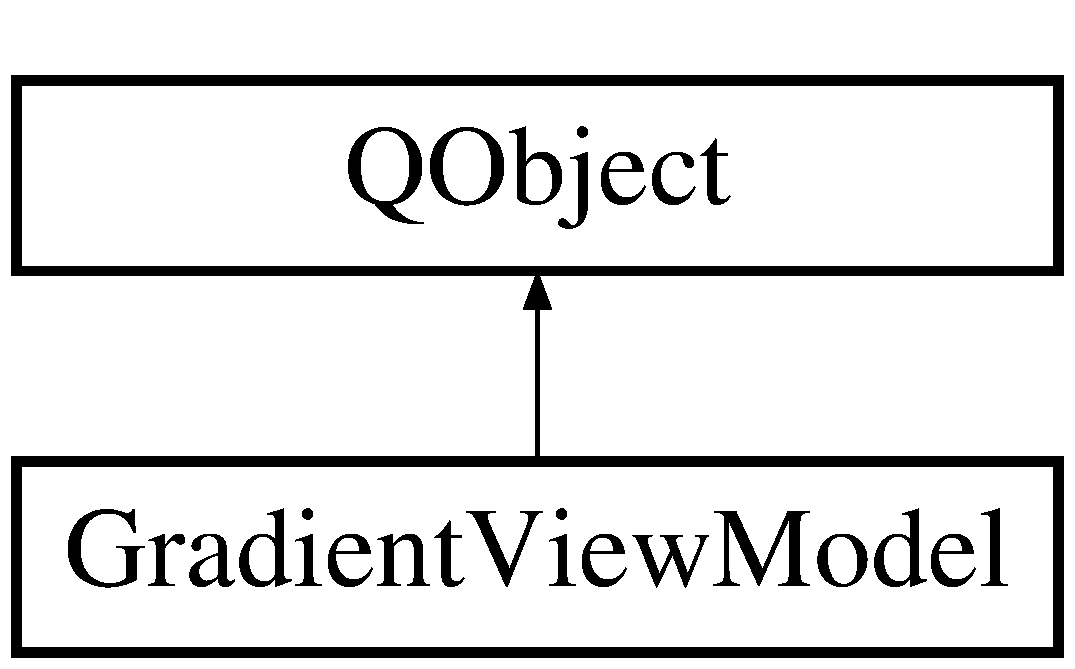
\includegraphics[height=2.000000cm]{class_gradient_view_model}
\end{center}
\end{figure}
\subsection*{Sloty publiczne}
\begin{DoxyCompactItemize}
\item 
void \mbox{\hyperlink{class_gradient_view_model_a44a264b3dfb259c75107dd80b1d7e389}{set\+Gradient\+Vector}} (Q\+Vector$<$ Q\+String $>$ vect)
\begin{DoxyCompactList}\small\item\em set\+Gradient\+Vector Modyfikuje właściwość gradient\+Vector \end{DoxyCompactList}\item 
void \mbox{\hyperlink{class_gradient_view_model_a17f428fa2bb8885ecf5e712e1d35c7a8}{set\+Selected\+Diode}} (int diode)
\begin{DoxyCompactList}\small\item\em set\+Selected\+Diode Modyfikuje właściwość selected\+Diode \end{DoxyCompactList}\item 
void \mbox{\hyperlink{class_gradient_view_model_ad90c266ab078a0701788f2a7a9c7f2be}{set\+Selected\+Type}} (int type)
\begin{DoxyCompactList}\small\item\em set\+Selected\+Type Modyfikuje właściwość selected\+Type, wywołuje konwersję między przestrzeniami H\+SV i R\+GB \end{DoxyCompactList}\item 
void \mbox{\hyperlink{class_gradient_view_model_a1a5a60c3fb1224b70203f811747043c1}{Set\+RH}} (int color)
\begin{DoxyCompactList}\small\item\em Set\+RH Modyfikuje właściwość RH. \end{DoxyCompactList}\item 
void \mbox{\hyperlink{class_gradient_view_model_a2b2cd55164016c051b0784396b51c0eb}{Set\+GS}} (int color)
\begin{DoxyCompactList}\small\item\em Set\+GS Modyfikuje właściwość GS. \end{DoxyCompactList}\item 
void \mbox{\hyperlink{class_gradient_view_model_a20989bc2daaea85e5cc33513af1b2660}{Set\+BV}} (int color)
\begin{DoxyCompactList}\small\item\em Set\+BV Modyfikuje właściwość BV. \end{DoxyCompactList}\end{DoxyCompactItemize}
\subsection*{Sygnały}
\begin{DoxyCompactItemize}
\item 
void \mbox{\hyperlink{class_gradient_view_model_a5f33840baf0a02fab681992c3a9fbb29}{gradient\+Vector\+Changed}} (Q\+Vector$<$ Q\+String $>$ arg)
\begin{DoxyCompactList}\small\item\em gradient\+Vector\+Changed Informuje o zmianie elementów kolekcji \end{DoxyCompactList}\item 
void \mbox{\hyperlink{class_gradient_view_model_ad26d1979a011e1810e3e2e6c648b3882}{selected\+Diode\+Changed}} (int arg)
\begin{DoxyCompactList}\small\item\em selected\+Diode\+Changed Informuje o zmianie wybranego końca gradientu \end{DoxyCompactList}\item 
void \mbox{\hyperlink{class_gradient_view_model_a5dbe7b881e5b4ef1ddbed14f0015a355}{selected\+Type\+Changed}} (int arg)
\begin{DoxyCompactList}\small\item\em selected\+Type\+Changed Informuje o zmianie wybranej przestrzeni barw \end{DoxyCompactList}\item 
void \mbox{\hyperlink{class_gradient_view_model_a50c4f64eb680f0efdb80b1e6888fc51c}{R\+H\+Changed}} (int arg)
\begin{DoxyCompactList}\small\item\em R\+H\+Changed Informuje o zmianie właściwości RH. \end{DoxyCompactList}\item 
void \mbox{\hyperlink{class_gradient_view_model_a09e3fbfaa0b3f501ae7637736b5dcdc5}{G\+S\+Changed}} (int arg)
\begin{DoxyCompactList}\small\item\em G\+S\+Changed Informuje o zmianie właściwości GS. \end{DoxyCompactList}\item 
void \mbox{\hyperlink{class_gradient_view_model_affb6254ecc82d22552db80ecb959a9a0}{B\+V\+Changed}} (int arg)
\begin{DoxyCompactList}\small\item\em selected\+Type\+Changed Informuje o zmianie wybranej przestrzeni barw \end{DoxyCompactList}\end{DoxyCompactItemize}
\subsection*{Metody publiczne}
\begin{DoxyCompactItemize}
\item 
\mbox{\Hypertarget{class_gradient_view_model_a4cb2509cf74f45c66ae720ac3a6429f1}\label{class_gradient_view_model_a4cb2509cf74f45c66ae720ac3a6429f1}} 
{\bfseries Gradient\+View\+Model} (Q\+Object $\ast$parent=nullptr)
\item 
Q\+Vector$<$ Q\+String $>$ \mbox{\hyperlink{class_gradient_view_model_a267819ee342ee0d7b8d59a07eca2f44a}{get\+Gradient\+Vector}} ()
\begin{DoxyCompactList}\small\item\em get\+Gradient\+Vector \end{DoxyCompactList}\item 
int \mbox{\hyperlink{class_gradient_view_model_afbe2bb56ec39369736a0e4969a94de5b}{get\+Selected\+Diode}} ()
\begin{DoxyCompactList}\small\item\em get\+Selected\+Diode \end{DoxyCompactList}\item 
int \mbox{\hyperlink{class_gradient_view_model_a44e6045ecb0d0ee9a9ab775e97ddf33c}{get\+Selected\+Type}} ()
\begin{DoxyCompactList}\small\item\em get\+Selected\+Type \end{DoxyCompactList}\item 
int \mbox{\hyperlink{class_gradient_view_model_af2ca9997921048e2ded10b40fd947ae5}{Get\+RH}} ()
\begin{DoxyCompactList}\small\item\em Get\+RH. \end{DoxyCompactList}\item 
int \mbox{\hyperlink{class_gradient_view_model_a2df0db48205c8f0f7c72743c1a5f960d}{Get\+GS}} ()
\begin{DoxyCompactList}\small\item\em Get\+GS. \end{DoxyCompactList}\item 
int \mbox{\hyperlink{class_gradient_view_model_ac3643df9744d6672719c7d15d9d8a544}{Get\+BV}} ()
\begin{DoxyCompactList}\small\item\em Get\+BV. \end{DoxyCompactList}\item 
\mbox{\Hypertarget{class_gradient_view_model_a51315c70cc18585c645e05dcc73e6c57}\label{class_gradient_view_model_a51315c70cc18585c645e05dcc73e6c57}} 
Q\+\_\+\+I\+N\+V\+O\+K\+A\+B\+LE void \mbox{\hyperlink{class_gradient_view_model_a51315c70cc18585c645e05dcc73e6c57}{Send\+Gradient}} ()
\begin{DoxyCompactList}\small\item\em Metoda wysyła dane na temat wybranych kolorów do urządzenia. \end{DoxyCompactList}\end{DoxyCompactItemize}
\subsection*{Właściwości}
\begin{DoxyCompactItemize}
\item 
\mbox{\Hypertarget{class_gradient_view_model_a53c45ee55828896e8da5541aee55f010}\label{class_gradient_view_model_a53c45ee55828896e8da5541aee55f010}} 
Q\+Vector$<$ Q\+String $>$ {\bfseries gradient\+Vector}
\item 
\mbox{\Hypertarget{class_gradient_view_model_a99b38588ddd7327b24edb9a1949af53e}\label{class_gradient_view_model_a99b38588ddd7327b24edb9a1949af53e}} 
int {\bfseries selected\+Diode}
\item 
\mbox{\Hypertarget{class_gradient_view_model_a8f59afe82a71f2b62e35d3f7f28c7d7a}\label{class_gradient_view_model_a8f59afe82a71f2b62e35d3f7f28c7d7a}} 
int {\bfseries selected\+Type}
\item 
\mbox{\Hypertarget{class_gradient_view_model_a1f5d000e7a1a24d86b59fbbc6e10892e}\label{class_gradient_view_model_a1f5d000e7a1a24d86b59fbbc6e10892e}} 
int {\bfseries RH}
\item 
\mbox{\Hypertarget{class_gradient_view_model_acb5ce2894831c795264a7a3130b4dd52}\label{class_gradient_view_model_acb5ce2894831c795264a7a3130b4dd52}} 
int {\bfseries GS}
\item 
\mbox{\Hypertarget{class_gradient_view_model_ac7d5d88278017448e6a259308e1652f5}\label{class_gradient_view_model_ac7d5d88278017448e6a259308e1652f5}} 
int {\bfseries BV}
\end{DoxyCompactItemize}


\subsection{Opis szczegółowy}
The \mbox{\hyperlink{class_gradient_view_model}{Gradient\+View\+Model}} class Klasa pozwala na obsługę tworzenia gradientu dwukolorowego. 

\subsection{Dokumentacja funkcji składowych}
\mbox{\Hypertarget{class_gradient_view_model_affb6254ecc82d22552db80ecb959a9a0}\label{class_gradient_view_model_affb6254ecc82d22552db80ecb959a9a0}} 
\index{Gradient\+View\+Model@{Gradient\+View\+Model}!B\+V\+Changed@{B\+V\+Changed}}
\index{B\+V\+Changed@{B\+V\+Changed}!Gradient\+View\+Model@{Gradient\+View\+Model}}
\subsubsection{\texorpdfstring{B\+V\+Changed}{BVChanged}}
{\footnotesize\ttfamily void Gradient\+View\+Model\+::\+B\+V\+Changed (\begin{DoxyParamCaption}\item[{int}]{arg }\end{DoxyParamCaption})\hspace{0.3cm}{\ttfamily [signal]}}



selected\+Type\+Changed Informuje o zmianie wybranej przestrzeni barw 


\begin{DoxyParams}{Parametry}
{\em arg} & numer indeksu odpowiadającego wybranej przestrzeni barw \\
\hline
\end{DoxyParams}
\mbox{\Hypertarget{class_gradient_view_model_ac3643df9744d6672719c7d15d9d8a544}\label{class_gradient_view_model_ac3643df9744d6672719c7d15d9d8a544}} 
\index{Gradient\+View\+Model@{Gradient\+View\+Model}!Get\+BV@{Get\+BV}}
\index{Get\+BV@{Get\+BV}!Gradient\+View\+Model@{Gradient\+View\+Model}}
\subsubsection{\texorpdfstring{Get\+B\+V()}{GetBV()}}
{\footnotesize\ttfamily int Gradient\+View\+Model\+::\+Get\+BV (\begin{DoxyParamCaption}{ }\end{DoxyParamCaption})}



Get\+BV. 

\begin{DoxyReturn}{Zwraca}
wartość składowej Blue lub Value wybranego końca gradientu 
\end{DoxyReturn}
\mbox{\Hypertarget{class_gradient_view_model_a267819ee342ee0d7b8d59a07eca2f44a}\label{class_gradient_view_model_a267819ee342ee0d7b8d59a07eca2f44a}} 
\index{Gradient\+View\+Model@{Gradient\+View\+Model}!get\+Gradient\+Vector@{get\+Gradient\+Vector}}
\index{get\+Gradient\+Vector@{get\+Gradient\+Vector}!Gradient\+View\+Model@{Gradient\+View\+Model}}
\subsubsection{\texorpdfstring{get\+Gradient\+Vector()}{getGradientVector()}}
{\footnotesize\ttfamily Q\+Vector$<$ Q\+String $>$ Gradient\+View\+Model\+::get\+Gradient\+Vector (\begin{DoxyParamCaption}{ }\end{DoxyParamCaption})}



get\+Gradient\+Vector 

\begin{DoxyReturn}{Zwraca}
kolekcja kodów szesnastkowych kolorów 
\end{DoxyReturn}
\mbox{\Hypertarget{class_gradient_view_model_a2df0db48205c8f0f7c72743c1a5f960d}\label{class_gradient_view_model_a2df0db48205c8f0f7c72743c1a5f960d}} 
\index{Gradient\+View\+Model@{Gradient\+View\+Model}!Get\+GS@{Get\+GS}}
\index{Get\+GS@{Get\+GS}!Gradient\+View\+Model@{Gradient\+View\+Model}}
\subsubsection{\texorpdfstring{Get\+G\+S()}{GetGS()}}
{\footnotesize\ttfamily int Gradient\+View\+Model\+::\+Get\+GS (\begin{DoxyParamCaption}{ }\end{DoxyParamCaption})}



Get\+GS. 

\begin{DoxyReturn}{Zwraca}
wartość składowej Green lub Saturation wybranego końca gradientu 
\end{DoxyReturn}
\mbox{\Hypertarget{class_gradient_view_model_af2ca9997921048e2ded10b40fd947ae5}\label{class_gradient_view_model_af2ca9997921048e2ded10b40fd947ae5}} 
\index{Gradient\+View\+Model@{Gradient\+View\+Model}!Get\+RH@{Get\+RH}}
\index{Get\+RH@{Get\+RH}!Gradient\+View\+Model@{Gradient\+View\+Model}}
\subsubsection{\texorpdfstring{Get\+R\+H()}{GetRH()}}
{\footnotesize\ttfamily int Gradient\+View\+Model\+::\+Get\+RH (\begin{DoxyParamCaption}{ }\end{DoxyParamCaption})}



Get\+RH. 

\begin{DoxyReturn}{Zwraca}
wartość składowej Red lub Hue wybranego końca gradientu 
\end{DoxyReturn}
\mbox{\Hypertarget{class_gradient_view_model_afbe2bb56ec39369736a0e4969a94de5b}\label{class_gradient_view_model_afbe2bb56ec39369736a0e4969a94de5b}} 
\index{Gradient\+View\+Model@{Gradient\+View\+Model}!get\+Selected\+Diode@{get\+Selected\+Diode}}
\index{get\+Selected\+Diode@{get\+Selected\+Diode}!Gradient\+View\+Model@{Gradient\+View\+Model}}
\subsubsection{\texorpdfstring{get\+Selected\+Diode()}{getSelectedDiode()}}
{\footnotesize\ttfamily int Gradient\+View\+Model\+::get\+Selected\+Diode (\begin{DoxyParamCaption}{ }\end{DoxyParamCaption})}



get\+Selected\+Diode 

\begin{DoxyReturn}{Zwraca}
indeks wybranego końca gradientu 
\end{DoxyReturn}
\mbox{\Hypertarget{class_gradient_view_model_a44e6045ecb0d0ee9a9ab775e97ddf33c}\label{class_gradient_view_model_a44e6045ecb0d0ee9a9ab775e97ddf33c}} 
\index{Gradient\+View\+Model@{Gradient\+View\+Model}!get\+Selected\+Type@{get\+Selected\+Type}}
\index{get\+Selected\+Type@{get\+Selected\+Type}!Gradient\+View\+Model@{Gradient\+View\+Model}}
\subsubsection{\texorpdfstring{get\+Selected\+Type()}{getSelectedType()}}
{\footnotesize\ttfamily int Gradient\+View\+Model\+::get\+Selected\+Type (\begin{DoxyParamCaption}{ }\end{DoxyParamCaption})}



get\+Selected\+Type 

\begin{DoxyReturn}{Zwraca}
indeks wybranej przestrzeni barw 
\end{DoxyReturn}
\mbox{\Hypertarget{class_gradient_view_model_a5f33840baf0a02fab681992c3a9fbb29}\label{class_gradient_view_model_a5f33840baf0a02fab681992c3a9fbb29}} 
\index{Gradient\+View\+Model@{Gradient\+View\+Model}!gradient\+Vector\+Changed@{gradient\+Vector\+Changed}}
\index{gradient\+Vector\+Changed@{gradient\+Vector\+Changed}!Gradient\+View\+Model@{Gradient\+View\+Model}}
\subsubsection{\texorpdfstring{gradient\+Vector\+Changed}{gradientVectorChanged}}
{\footnotesize\ttfamily void Gradient\+View\+Model\+::gradient\+Vector\+Changed (\begin{DoxyParamCaption}\item[{Q\+Vector$<$ Q\+String $>$}]{arg }\end{DoxyParamCaption})\hspace{0.3cm}{\ttfamily [signal]}}



gradient\+Vector\+Changed Informuje o zmianie elementów kolekcji 


\begin{DoxyParams}{Parametry}
{\em arg} & kolekcja kodów szesnastkowych kolorów gradientu \\
\hline
\end{DoxyParams}
\mbox{\Hypertarget{class_gradient_view_model_a09e3fbfaa0b3f501ae7637736b5dcdc5}\label{class_gradient_view_model_a09e3fbfaa0b3f501ae7637736b5dcdc5}} 
\index{Gradient\+View\+Model@{Gradient\+View\+Model}!G\+S\+Changed@{G\+S\+Changed}}
\index{G\+S\+Changed@{G\+S\+Changed}!Gradient\+View\+Model@{Gradient\+View\+Model}}
\subsubsection{\texorpdfstring{G\+S\+Changed}{GSChanged}}
{\footnotesize\ttfamily void Gradient\+View\+Model\+::\+G\+S\+Changed (\begin{DoxyParamCaption}\item[{int}]{arg }\end{DoxyParamCaption})\hspace{0.3cm}{\ttfamily [signal]}}



G\+S\+Changed Informuje o zmianie właściwości GS. 


\begin{DoxyParams}{Parametry}
{\em arg} & wartość liczbowa składowej Green lub Saturation \\
\hline
\end{DoxyParams}
\mbox{\Hypertarget{class_gradient_view_model_a50c4f64eb680f0efdb80b1e6888fc51c}\label{class_gradient_view_model_a50c4f64eb680f0efdb80b1e6888fc51c}} 
\index{Gradient\+View\+Model@{Gradient\+View\+Model}!R\+H\+Changed@{R\+H\+Changed}}
\index{R\+H\+Changed@{R\+H\+Changed}!Gradient\+View\+Model@{Gradient\+View\+Model}}
\subsubsection{\texorpdfstring{R\+H\+Changed}{RHChanged}}
{\footnotesize\ttfamily void Gradient\+View\+Model\+::\+R\+H\+Changed (\begin{DoxyParamCaption}\item[{int}]{arg }\end{DoxyParamCaption})\hspace{0.3cm}{\ttfamily [signal]}}



R\+H\+Changed Informuje o zmianie właściwości RH. 


\begin{DoxyParams}{Parametry}
{\em arg} & wartość liczbowa składowej Red lub Hue \\
\hline
\end{DoxyParams}
\mbox{\Hypertarget{class_gradient_view_model_ad26d1979a011e1810e3e2e6c648b3882}\label{class_gradient_view_model_ad26d1979a011e1810e3e2e6c648b3882}} 
\index{Gradient\+View\+Model@{Gradient\+View\+Model}!selected\+Diode\+Changed@{selected\+Diode\+Changed}}
\index{selected\+Diode\+Changed@{selected\+Diode\+Changed}!Gradient\+View\+Model@{Gradient\+View\+Model}}
\subsubsection{\texorpdfstring{selected\+Diode\+Changed}{selectedDiodeChanged}}
{\footnotesize\ttfamily void Gradient\+View\+Model\+::selected\+Diode\+Changed (\begin{DoxyParamCaption}\item[{int}]{arg }\end{DoxyParamCaption})\hspace{0.3cm}{\ttfamily [signal]}}



selected\+Diode\+Changed Informuje o zmianie wybranego końca gradientu 


\begin{DoxyParams}{Parametry}
{\em arg} & indeks wybranego końca gradientu \\
\hline
\end{DoxyParams}
\mbox{\Hypertarget{class_gradient_view_model_a5dbe7b881e5b4ef1ddbed14f0015a355}\label{class_gradient_view_model_a5dbe7b881e5b4ef1ddbed14f0015a355}} 
\index{Gradient\+View\+Model@{Gradient\+View\+Model}!selected\+Type\+Changed@{selected\+Type\+Changed}}
\index{selected\+Type\+Changed@{selected\+Type\+Changed}!Gradient\+View\+Model@{Gradient\+View\+Model}}
\subsubsection{\texorpdfstring{selected\+Type\+Changed}{selectedTypeChanged}}
{\footnotesize\ttfamily void Gradient\+View\+Model\+::selected\+Type\+Changed (\begin{DoxyParamCaption}\item[{int}]{arg }\end{DoxyParamCaption})\hspace{0.3cm}{\ttfamily [signal]}}



selected\+Type\+Changed Informuje o zmianie wybranej przestrzeni barw 


\begin{DoxyParams}{Parametry}
{\em arg} & numer indeksu odpowiadającego wybranej przestrzeni barw \\
\hline
\end{DoxyParams}
\mbox{\Hypertarget{class_gradient_view_model_a20989bc2daaea85e5cc33513af1b2660}\label{class_gradient_view_model_a20989bc2daaea85e5cc33513af1b2660}} 
\index{Gradient\+View\+Model@{Gradient\+View\+Model}!Set\+BV@{Set\+BV}}
\index{Set\+BV@{Set\+BV}!Gradient\+View\+Model@{Gradient\+View\+Model}}
\subsubsection{\texorpdfstring{Set\+BV}{SetBV}}
{\footnotesize\ttfamily void Gradient\+View\+Model\+::\+Set\+BV (\begin{DoxyParamCaption}\item[{int}]{color }\end{DoxyParamCaption})\hspace{0.3cm}{\ttfamily [slot]}}



Set\+BV Modyfikuje właściwość BV. 


\begin{DoxyParams}{Parametry}
{\em bv} & wartość przypisywana właściwości BV \\
\hline
\end{DoxyParams}
\mbox{\Hypertarget{class_gradient_view_model_a44a264b3dfb259c75107dd80b1d7e389}\label{class_gradient_view_model_a44a264b3dfb259c75107dd80b1d7e389}} 
\index{Gradient\+View\+Model@{Gradient\+View\+Model}!set\+Gradient\+Vector@{set\+Gradient\+Vector}}
\index{set\+Gradient\+Vector@{set\+Gradient\+Vector}!Gradient\+View\+Model@{Gradient\+View\+Model}}
\subsubsection{\texorpdfstring{set\+Gradient\+Vector}{setGradientVector}}
{\footnotesize\ttfamily void Gradient\+View\+Model\+::set\+Gradient\+Vector (\begin{DoxyParamCaption}\item[{Q\+Vector$<$ Q\+String $>$}]{vect }\end{DoxyParamCaption})\hspace{0.3cm}{\ttfamily [slot]}}



set\+Gradient\+Vector Modyfikuje właściwość gradient\+Vector 


\begin{DoxyParams}{Parametry}
{\em vect} & kolekcja kodow szesnastkowych kolorów \\
\hline
\end{DoxyParams}
\mbox{\Hypertarget{class_gradient_view_model_a2b2cd55164016c051b0784396b51c0eb}\label{class_gradient_view_model_a2b2cd55164016c051b0784396b51c0eb}} 
\index{Gradient\+View\+Model@{Gradient\+View\+Model}!Set\+GS@{Set\+GS}}
\index{Set\+GS@{Set\+GS}!Gradient\+View\+Model@{Gradient\+View\+Model}}
\subsubsection{\texorpdfstring{Set\+GS}{SetGS}}
{\footnotesize\ttfamily void Gradient\+View\+Model\+::\+Set\+GS (\begin{DoxyParamCaption}\item[{int}]{color }\end{DoxyParamCaption})\hspace{0.3cm}{\ttfamily [slot]}}



Set\+GS Modyfikuje właściwość GS. 


\begin{DoxyParams}{Parametry}
{\em gs} & wartość przypisywana właściwości GS \\
\hline
\end{DoxyParams}
\mbox{\Hypertarget{class_gradient_view_model_a1a5a60c3fb1224b70203f811747043c1}\label{class_gradient_view_model_a1a5a60c3fb1224b70203f811747043c1}} 
\index{Gradient\+View\+Model@{Gradient\+View\+Model}!Set\+RH@{Set\+RH}}
\index{Set\+RH@{Set\+RH}!Gradient\+View\+Model@{Gradient\+View\+Model}}
\subsubsection{\texorpdfstring{Set\+RH}{SetRH}}
{\footnotesize\ttfamily void Gradient\+View\+Model\+::\+Set\+RH (\begin{DoxyParamCaption}\item[{int}]{color }\end{DoxyParamCaption})\hspace{0.3cm}{\ttfamily [slot]}}



Set\+RH Modyfikuje właściwość RH. 


\begin{DoxyParams}{Parametry}
{\em rh} & wartość przypisywana właściwości RH \\
\hline
\end{DoxyParams}
\mbox{\Hypertarget{class_gradient_view_model_a17f428fa2bb8885ecf5e712e1d35c7a8}\label{class_gradient_view_model_a17f428fa2bb8885ecf5e712e1d35c7a8}} 
\index{Gradient\+View\+Model@{Gradient\+View\+Model}!set\+Selected\+Diode@{set\+Selected\+Diode}}
\index{set\+Selected\+Diode@{set\+Selected\+Diode}!Gradient\+View\+Model@{Gradient\+View\+Model}}
\subsubsection{\texorpdfstring{set\+Selected\+Diode}{setSelectedDiode}}
{\footnotesize\ttfamily void Gradient\+View\+Model\+::set\+Selected\+Diode (\begin{DoxyParamCaption}\item[{int}]{diode }\end{DoxyParamCaption})\hspace{0.3cm}{\ttfamily [slot]}}



set\+Selected\+Diode Modyfikuje właściwość selected\+Diode 


\begin{DoxyParams}{Parametry}
{\em diode} & indeks wybieranego końca gradientu \\
\hline
\end{DoxyParams}
\mbox{\Hypertarget{class_gradient_view_model_ad90c266ab078a0701788f2a7a9c7f2be}\label{class_gradient_view_model_ad90c266ab078a0701788f2a7a9c7f2be}} 
\index{Gradient\+View\+Model@{Gradient\+View\+Model}!set\+Selected\+Type@{set\+Selected\+Type}}
\index{set\+Selected\+Type@{set\+Selected\+Type}!Gradient\+View\+Model@{Gradient\+View\+Model}}
\subsubsection{\texorpdfstring{set\+Selected\+Type}{setSelectedType}}
{\footnotesize\ttfamily void Gradient\+View\+Model\+::set\+Selected\+Type (\begin{DoxyParamCaption}\item[{int}]{type }\end{DoxyParamCaption})\hspace{0.3cm}{\ttfamily [slot]}}



set\+Selected\+Type Modyfikuje właściwość selected\+Type, wywołuje konwersję między przestrzeniami H\+SV i R\+GB 


\begin{DoxyParams}{Parametry}
{\em selection} & numer indeksu odpowiadającego wybranej przestrzeni barw \\
\hline
\end{DoxyParams}


Dokumentacja dla tej klasy została wygenerowana z plików\+:\begin{DoxyCompactItemize}
\item 
C\+:/\+Users/amy1/\+Source/\+Qt/\+Lampki\+App/\+View\+Models/gradientviewmodel.\+h\item 
C\+:/\+Users/amy1/\+Source/\+Qt/\+Lampki\+App/\+View\+Models/gradientviewmodel.\+cpp\end{DoxyCompactItemize}

\hypertarget{class_h_s_v_color_model}{}\section{Dokumentacja klasy H\+S\+V\+Color\+Model}
\label{class_h_s_v_color_model}\index{H\+S\+V\+Color\+Model@{H\+S\+V\+Color\+Model}}


The \mbox{\hyperlink{class_h_s_v_color_model}{H\+S\+V\+Color\+Model}} class Klasa dziedziczy po abstrakcyjnej klasie \mbox{\hyperlink{class_a_color_model}{A\+Color\+Model}}. Odpowiada za przetwarzanie danych dotyczacych koloru w przestrzeni barw H\+SV.  




{\ttfamily \#include $<$hsvcolormodel.\+h$>$}

Diagram dziedziczenia dla H\+S\+V\+Color\+Model\begin{figure}[H]
\begin{center}
\leavevmode
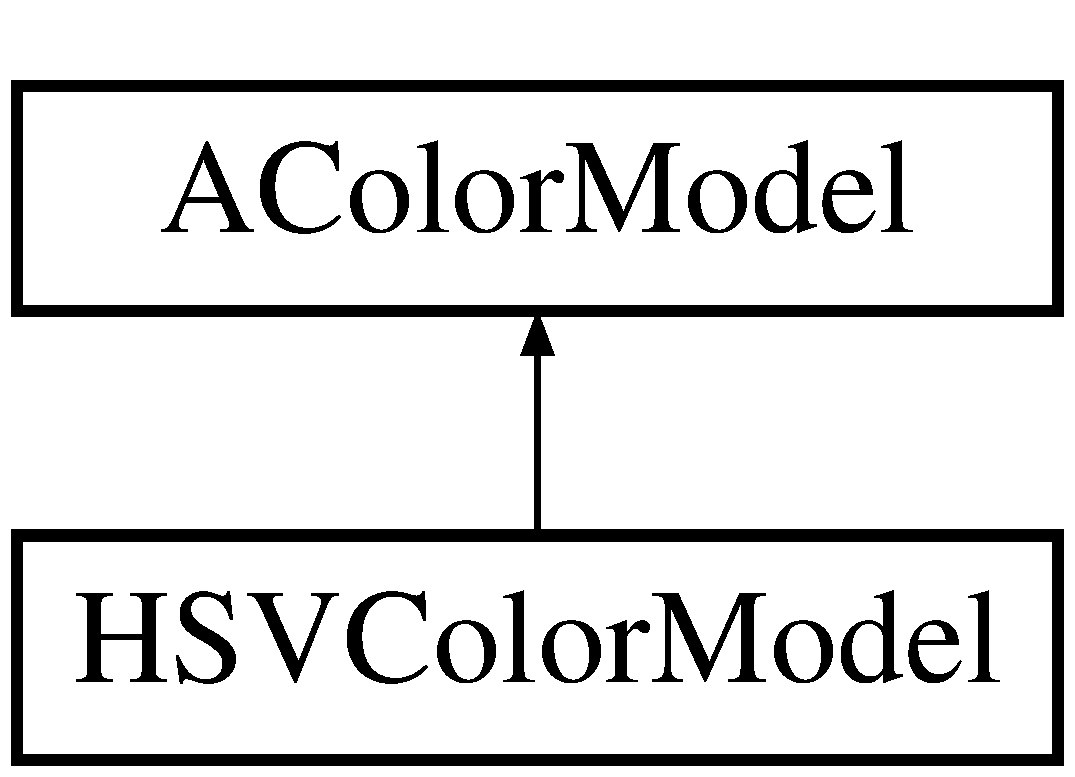
\includegraphics[height=2.000000cm]{class_h_s_v_color_model}
\end{center}
\end{figure}
\subsection*{Metody publiczne}
\begin{DoxyCompactItemize}
\item 
\mbox{\hyperlink{class_h_s_v_color_model_a7dac5687cef8207ebc8279414cfa6706}{H\+S\+V\+Color\+Model}} (int h, int s, int v)
\begin{DoxyCompactList}\small\item\em \mbox{\hyperlink{class_h_s_v_color_model}{H\+S\+V\+Color\+Model}} Inicjalizuje obiekt klasy \mbox{\hyperlink{class_h_s_v_color_model}{H\+S\+V\+Color\+Model}}. \end{DoxyCompactList}\item 
std\+::unique\+\_\+ptr$<$ \mbox{\hyperlink{class_a_color_model}{A\+Color\+Model}} $>$ \mbox{\hyperlink{class_h_s_v_color_model_a576aa9888f81248c99e67da6bb0587d2}{As\+R\+GB}} () override
\begin{DoxyCompactList}\small\item\em As\+R\+GB Metoda wywołuje metodę parsującą Parse\+To\+R\+G\+B() i zwraca wynik konwersji. \end{DoxyCompactList}\item 
std\+::unique\+\_\+ptr$<$ \mbox{\hyperlink{class_a_color_model}{A\+Color\+Model}} $>$ \mbox{\hyperlink{class_h_s_v_color_model_a4f15c9e48f157f7bd83f5a0837f1ac87}{As\+H\+SV}} () override
\begin{DoxyCompactList}\small\item\em As\+H\+SV Metoda przekazuje obiekt klasy \mbox{\hyperlink{class_h_s_v_color_model}{H\+S\+V\+Color\+Model}}. \end{DoxyCompactList}\item 
Q\+String \mbox{\hyperlink{class_h_s_v_color_model_ab67eb5960aa53f4b573c40fd0945a9b9}{As\+Hex}} ()
\begin{DoxyCompactList}\small\item\em As\+Hex Metoda wykonuje konwersję do modelu R\+GB, następnie przy użyciu String\+Stream wartości składowe konwertowane są do systemu heksadecymmalnego oraz łączone w kod szesnastkowy danego koloru. \end{DoxyCompactList}\item 
int \mbox{\hyperlink{class_h_s_v_color_model_aeb9fd06a7806c227ee6a8ad85ee9fbf8}{Get\+RH}} () override
\begin{DoxyCompactList}\small\item\em Get\+RH. \end{DoxyCompactList}\item 
int \mbox{\hyperlink{class_h_s_v_color_model_a458ef47bbc34635460fe2d51ddbb858b}{Get\+GS}} () override
\begin{DoxyCompactList}\small\item\em Get\+GS. \end{DoxyCompactList}\item 
int \mbox{\hyperlink{class_h_s_v_color_model_a9365e20ba9a7eeccecc17ef7494b721a}{Get\+BV}} () override
\begin{DoxyCompactList}\small\item\em Get\+BV. \end{DoxyCompactList}\item 
void \mbox{\hyperlink{class_h_s_v_color_model_ae451a6fb2bd74cea52f96810e0140d46}{Set\+RH}} (int rh) override
\begin{DoxyCompactList}\small\item\em Set\+RH Modyfikuje wartość pola hue. \end{DoxyCompactList}\item 
void \mbox{\hyperlink{class_h_s_v_color_model_a3478cc455994e6b0737391e083f1666a}{Set\+GS}} (int gs) override
\begin{DoxyCompactList}\small\item\em Set\+GS Modyfikuje wartość pola saturation. \end{DoxyCompactList}\item 
void \mbox{\hyperlink{class_h_s_v_color_model_a4213b3b016d213e791b97438e62c9c1f}{Set\+BV}} (int bv) override
\begin{DoxyCompactList}\small\item\em Set\+BV Modyfikuje wartość pola value. \end{DoxyCompactList}\end{DoxyCompactItemize}


\subsection{Opis szczegółowy}
The \mbox{\hyperlink{class_h_s_v_color_model}{H\+S\+V\+Color\+Model}} class Klasa dziedziczy po abstrakcyjnej klasie \mbox{\hyperlink{class_a_color_model}{A\+Color\+Model}}. Odpowiada za przetwarzanie danych dotyczacych koloru w przestrzeni barw H\+SV. 

\subsection{Dokumentacja konstruktora i destruktora}
\mbox{\Hypertarget{class_h_s_v_color_model_a7dac5687cef8207ebc8279414cfa6706}\label{class_h_s_v_color_model_a7dac5687cef8207ebc8279414cfa6706}} 
\index{H\+S\+V\+Color\+Model@{H\+S\+V\+Color\+Model}!H\+S\+V\+Color\+Model@{H\+S\+V\+Color\+Model}}
\index{H\+S\+V\+Color\+Model@{H\+S\+V\+Color\+Model}!H\+S\+V\+Color\+Model@{H\+S\+V\+Color\+Model}}
\subsubsection{\texorpdfstring{H\+S\+V\+Color\+Model()}{HSVColorModel()}}
{\footnotesize\ttfamily H\+S\+V\+Color\+Model\+::\+H\+S\+V\+Color\+Model (\begin{DoxyParamCaption}\item[{int}]{h,  }\item[{int}]{s,  }\item[{int}]{v }\end{DoxyParamCaption})}



\mbox{\hyperlink{class_h_s_v_color_model}{H\+S\+V\+Color\+Model}} Inicjalizuje obiekt klasy \mbox{\hyperlink{class_h_s_v_color_model}{H\+S\+V\+Color\+Model}}. 


\begin{DoxyParams}{Parametry}
{\em h} & Wartość do zainicjalizowania pola hue \\
\hline
{\em s} & Wartość do zainicjalizowania pola saturation \\
\hline
{\em v} & Wartość do zainicjalizowania pola value \\
\hline
\end{DoxyParams}


\subsection{Dokumentacja funkcji składowych}
\mbox{\Hypertarget{class_h_s_v_color_model_ab67eb5960aa53f4b573c40fd0945a9b9}\label{class_h_s_v_color_model_ab67eb5960aa53f4b573c40fd0945a9b9}} 
\index{H\+S\+V\+Color\+Model@{H\+S\+V\+Color\+Model}!As\+Hex@{As\+Hex}}
\index{As\+Hex@{As\+Hex}!H\+S\+V\+Color\+Model@{H\+S\+V\+Color\+Model}}
\subsubsection{\texorpdfstring{As\+Hex()}{AsHex()}}
{\footnotesize\ttfamily Q\+String H\+S\+V\+Color\+Model\+::\+As\+Hex (\begin{DoxyParamCaption}{ }\end{DoxyParamCaption})\hspace{0.3cm}{\ttfamily [virtual]}}



As\+Hex Metoda wykonuje konwersję do modelu R\+GB, następnie przy użyciu String\+Stream wartości składowe konwertowane są do systemu heksadecymmalnego oraz łączone w kod szesnastkowy danego koloru. 

\begin{DoxyReturn}{Zwraca}
Q\+String zawierający kod szesnastkowy koloru 
\end{DoxyReturn}


Implementuje \mbox{\hyperlink{class_a_color_model}{A\+Color\+Model}}.

\mbox{\Hypertarget{class_h_s_v_color_model_a4f15c9e48f157f7bd83f5a0837f1ac87}\label{class_h_s_v_color_model_a4f15c9e48f157f7bd83f5a0837f1ac87}} 
\index{H\+S\+V\+Color\+Model@{H\+S\+V\+Color\+Model}!As\+H\+SV@{As\+H\+SV}}
\index{As\+H\+SV@{As\+H\+SV}!H\+S\+V\+Color\+Model@{H\+S\+V\+Color\+Model}}
\subsubsection{\texorpdfstring{As\+H\+S\+V()}{AsHSV()}}
{\footnotesize\ttfamily std\+::unique\+\_\+ptr$<$ \mbox{\hyperlink{class_a_color_model}{A\+Color\+Model}} $>$ H\+S\+V\+Color\+Model\+::\+As\+H\+SV (\begin{DoxyParamCaption}{ }\end{DoxyParamCaption})\hspace{0.3cm}{\ttfamily [override]}, {\ttfamily [virtual]}}



As\+H\+SV Metoda przekazuje obiekt klasy \mbox{\hyperlink{class_h_s_v_color_model}{H\+S\+V\+Color\+Model}}. 

\begin{DoxyReturn}{Zwraca}
unique\+\_\+ptr do obiektu klasy \mbox{\hyperlink{class_h_s_v_color_model}{H\+S\+V\+Color\+Model}} 
\end{DoxyReturn}


Implementuje \mbox{\hyperlink{class_a_color_model}{A\+Color\+Model}}.

\mbox{\Hypertarget{class_h_s_v_color_model_a576aa9888f81248c99e67da6bb0587d2}\label{class_h_s_v_color_model_a576aa9888f81248c99e67da6bb0587d2}} 
\index{H\+S\+V\+Color\+Model@{H\+S\+V\+Color\+Model}!As\+R\+GB@{As\+R\+GB}}
\index{As\+R\+GB@{As\+R\+GB}!H\+S\+V\+Color\+Model@{H\+S\+V\+Color\+Model}}
\subsubsection{\texorpdfstring{As\+R\+G\+B()}{AsRGB()}}
{\footnotesize\ttfamily std\+::unique\+\_\+ptr$<$ \mbox{\hyperlink{class_a_color_model}{A\+Color\+Model}} $>$ H\+S\+V\+Color\+Model\+::\+As\+R\+GB (\begin{DoxyParamCaption}{ }\end{DoxyParamCaption})\hspace{0.3cm}{\ttfamily [override]}, {\ttfamily [virtual]}}



As\+R\+GB Metoda wywołuje metodę parsującą Parse\+To\+R\+G\+B() i zwraca wynik konwersji. 

\begin{DoxyReturn}{Zwraca}
unique\+\_\+ptr do obiektu klasy \mbox{\hyperlink{class_r_g_b_color_model}{R\+G\+B\+Color\+Model}} 
\end{DoxyReturn}


Implementuje \mbox{\hyperlink{class_a_color_model}{A\+Color\+Model}}.

\mbox{\Hypertarget{class_h_s_v_color_model_a9365e20ba9a7eeccecc17ef7494b721a}\label{class_h_s_v_color_model_a9365e20ba9a7eeccecc17ef7494b721a}} 
\index{H\+S\+V\+Color\+Model@{H\+S\+V\+Color\+Model}!Get\+BV@{Get\+BV}}
\index{Get\+BV@{Get\+BV}!H\+S\+V\+Color\+Model@{H\+S\+V\+Color\+Model}}
\subsubsection{\texorpdfstring{Get\+B\+V()}{GetBV()}}
{\footnotesize\ttfamily int H\+S\+V\+Color\+Model\+::\+Get\+BV (\begin{DoxyParamCaption}{ }\end{DoxyParamCaption})\hspace{0.3cm}{\ttfamily [override]}, {\ttfamily [virtual]}}



Get\+BV. 

\begin{DoxyReturn}{Zwraca}
wartość pola value 
\end{DoxyReturn}


Implementuje \mbox{\hyperlink{class_a_color_model}{A\+Color\+Model}}.

\mbox{\Hypertarget{class_h_s_v_color_model_a458ef47bbc34635460fe2d51ddbb858b}\label{class_h_s_v_color_model_a458ef47bbc34635460fe2d51ddbb858b}} 
\index{H\+S\+V\+Color\+Model@{H\+S\+V\+Color\+Model}!Get\+GS@{Get\+GS}}
\index{Get\+GS@{Get\+GS}!H\+S\+V\+Color\+Model@{H\+S\+V\+Color\+Model}}
\subsubsection{\texorpdfstring{Get\+G\+S()}{GetGS()}}
{\footnotesize\ttfamily int H\+S\+V\+Color\+Model\+::\+Get\+GS (\begin{DoxyParamCaption}{ }\end{DoxyParamCaption})\hspace{0.3cm}{\ttfamily [override]}, {\ttfamily [virtual]}}



Get\+GS. 

\begin{DoxyReturn}{Zwraca}
wartość pola saturation 
\end{DoxyReturn}


Implementuje \mbox{\hyperlink{class_a_color_model}{A\+Color\+Model}}.

\mbox{\Hypertarget{class_h_s_v_color_model_aeb9fd06a7806c227ee6a8ad85ee9fbf8}\label{class_h_s_v_color_model_aeb9fd06a7806c227ee6a8ad85ee9fbf8}} 
\index{H\+S\+V\+Color\+Model@{H\+S\+V\+Color\+Model}!Get\+RH@{Get\+RH}}
\index{Get\+RH@{Get\+RH}!H\+S\+V\+Color\+Model@{H\+S\+V\+Color\+Model}}
\subsubsection{\texorpdfstring{Get\+R\+H()}{GetRH()}}
{\footnotesize\ttfamily int H\+S\+V\+Color\+Model\+::\+Get\+RH (\begin{DoxyParamCaption}{ }\end{DoxyParamCaption})\hspace{0.3cm}{\ttfamily [override]}, {\ttfamily [virtual]}}



Get\+RH. 

\begin{DoxyReturn}{Zwraca}
wartość pola hue 
\end{DoxyReturn}


Implementuje \mbox{\hyperlink{class_a_color_model}{A\+Color\+Model}}.

\mbox{\Hypertarget{class_h_s_v_color_model_a4213b3b016d213e791b97438e62c9c1f}\label{class_h_s_v_color_model_a4213b3b016d213e791b97438e62c9c1f}} 
\index{H\+S\+V\+Color\+Model@{H\+S\+V\+Color\+Model}!Set\+BV@{Set\+BV}}
\index{Set\+BV@{Set\+BV}!H\+S\+V\+Color\+Model@{H\+S\+V\+Color\+Model}}
\subsubsection{\texorpdfstring{Set\+B\+V()}{SetBV()}}
{\footnotesize\ttfamily void H\+S\+V\+Color\+Model\+::\+Set\+BV (\begin{DoxyParamCaption}\item[{int}]{bv }\end{DoxyParamCaption})\hspace{0.3cm}{\ttfamily [override]}, {\ttfamily [virtual]}}



Set\+BV Modyfikuje wartość pola value. 


\begin{DoxyParams}{Parametry}
{\em bv} & Wartość przypisywana składowej value \\
\hline
\end{DoxyParams}


Implementuje \mbox{\hyperlink{class_a_color_model}{A\+Color\+Model}}.

\mbox{\Hypertarget{class_h_s_v_color_model_a3478cc455994e6b0737391e083f1666a}\label{class_h_s_v_color_model_a3478cc455994e6b0737391e083f1666a}} 
\index{H\+S\+V\+Color\+Model@{H\+S\+V\+Color\+Model}!Set\+GS@{Set\+GS}}
\index{Set\+GS@{Set\+GS}!H\+S\+V\+Color\+Model@{H\+S\+V\+Color\+Model}}
\subsubsection{\texorpdfstring{Set\+G\+S()}{SetGS()}}
{\footnotesize\ttfamily void H\+S\+V\+Color\+Model\+::\+Set\+GS (\begin{DoxyParamCaption}\item[{int}]{gs }\end{DoxyParamCaption})\hspace{0.3cm}{\ttfamily [override]}, {\ttfamily [virtual]}}



Set\+GS Modyfikuje wartość pola saturation. 


\begin{DoxyParams}{Parametry}
{\em gs} & Wartośc przypisywana składowej saturation \\
\hline
\end{DoxyParams}


Implementuje \mbox{\hyperlink{class_a_color_model}{A\+Color\+Model}}.

\mbox{\Hypertarget{class_h_s_v_color_model_ae451a6fb2bd74cea52f96810e0140d46}\label{class_h_s_v_color_model_ae451a6fb2bd74cea52f96810e0140d46}} 
\index{H\+S\+V\+Color\+Model@{H\+S\+V\+Color\+Model}!Set\+RH@{Set\+RH}}
\index{Set\+RH@{Set\+RH}!H\+S\+V\+Color\+Model@{H\+S\+V\+Color\+Model}}
\subsubsection{\texorpdfstring{Set\+R\+H()}{SetRH()}}
{\footnotesize\ttfamily void H\+S\+V\+Color\+Model\+::\+Set\+RH (\begin{DoxyParamCaption}\item[{int}]{rh }\end{DoxyParamCaption})\hspace{0.3cm}{\ttfamily [override]}, {\ttfamily [virtual]}}



Set\+RH Modyfikuje wartość pola hue. 


\begin{DoxyParams}{Parametry}
{\em rh} & Wartość przypisywana składowej hue \\
\hline
\end{DoxyParams}


Implementuje \mbox{\hyperlink{class_a_color_model}{A\+Color\+Model}}.



Dokumentacja dla tej klasy została wygenerowana z plików\+:\begin{DoxyCompactItemize}
\item 
C\+:/\+Users/amy1/\+Source/\+Qt/\+Lampki\+App/\+Models/hsvcolormodel.\+h\item 
C\+:/\+Users/amy1/\+Source/\+Qt/\+Lampki\+App/\+Models/hsvcolormodel.\+cpp\end{DoxyCompactItemize}

\hypertarget{class_j_s_o_n_helper}{}\section{Dokumentacja klasy J\+S\+O\+N\+Helper}
\label{class_j_s_o_n_helper}\index{J\+S\+O\+N\+Helper@{J\+S\+O\+N\+Helper}}


The \mbox{\hyperlink{class_j_s_o_n_helper}{J\+S\+O\+N\+Helper}} class Klasa przygotowuje dane do przesłania poprzez zapisanie danych na temat ustawionych kolorów diod w Java\+Script Object Notation. Klasa jest zgodna z wzorcem Singleton.  




{\ttfamily \#include $<$jsonhelper.\+h$>$}

\subsection*{Metody publiczne}
\begin{DoxyCompactItemize}
\item 
Q\+Json\+Document \mbox{\hyperlink{class_j_s_o_n_helper_a4d4771c06547925f86cd02abba8af913}{Unicolor\+To\+Json}} (\mbox{\hyperlink{class_a_color_model}{A\+Color\+Model}} \&color)
\begin{DoxyCompactList}\small\item\em Unicolor\+To\+Json Tworzy J\+S\+O\+Na z kolorem wybranym w zakładce \char`\"{}\+Jeden kolor\char`\"{}. \end{DoxyCompactList}\item 
Q\+Json\+Document \mbox{\hyperlink{class_j_s_o_n_helper_ab31e0865df49879496cbc07232ceb8ce}{Multicolor\+To\+Json}} (Q\+Vector$<$ Q\+String $>$ color\+Array)
\begin{DoxyCompactList}\small\item\em Multicolor\+To\+Json Tworzy J\+S\+O\+Na z wieloma kolorami -\/ przypisanymi do każdej diody osobno. \end{DoxyCompactList}\end{DoxyCompactItemize}
\subsection*{Statyczne metody publiczne}
\begin{DoxyCompactItemize}
\item 
static \mbox{\hyperlink{class_j_s_o_n_helper}{J\+S\+O\+N\+Helper}} \& \mbox{\hyperlink{class_j_s_o_n_helper_a16b59ed7de044a5f3e81cc2109d370a1}{get\+Json\+Helper}} ()
\begin{DoxyCompactList}\small\item\em get\+Json\+Helper Zwraca referencję do istniejącego obiektu klasy lub inicjalizuje obiekt klasy \mbox{\hyperlink{class_j_s_o_n_helper}{J\+S\+O\+N\+Helper}}, jeśli nie został wcześniej utworzony \end{DoxyCompactList}\end{DoxyCompactItemize}


\subsection{Opis szczegółowy}
The \mbox{\hyperlink{class_j_s_o_n_helper}{J\+S\+O\+N\+Helper}} class Klasa przygotowuje dane do przesłania poprzez zapisanie danych na temat ustawionych kolorów diod w Java\+Script Object Notation. Klasa jest zgodna z wzorcem Singleton. 

\subsection{Dokumentacja funkcji składowych}
\mbox{\Hypertarget{class_j_s_o_n_helper_a16b59ed7de044a5f3e81cc2109d370a1}\label{class_j_s_o_n_helper_a16b59ed7de044a5f3e81cc2109d370a1}} 
\index{J\+S\+O\+N\+Helper@{J\+S\+O\+N\+Helper}!get\+Json\+Helper@{get\+Json\+Helper}}
\index{get\+Json\+Helper@{get\+Json\+Helper}!J\+S\+O\+N\+Helper@{J\+S\+O\+N\+Helper}}
\subsubsection{\texorpdfstring{get\+Json\+Helper()}{getJsonHelper()}}
{\footnotesize\ttfamily \mbox{\hyperlink{class_j_s_o_n_helper}{J\+S\+O\+N\+Helper}} \& J\+S\+O\+N\+Helper\+::get\+Json\+Helper (\begin{DoxyParamCaption}{ }\end{DoxyParamCaption})\hspace{0.3cm}{\ttfamily [static]}}



get\+Json\+Helper Zwraca referencję do istniejącego obiektu klasy lub inicjalizuje obiekt klasy \mbox{\hyperlink{class_j_s_o_n_helper}{J\+S\+O\+N\+Helper}}, jeśli nie został wcześniej utworzony 

\begin{DoxyReturn}{Zwraca}
referencja do obiektu klasy \mbox{\hyperlink{class_j_s_o_n_helper}{J\+S\+O\+N\+Helper}} 
\end{DoxyReturn}
\mbox{\Hypertarget{class_j_s_o_n_helper_ab31e0865df49879496cbc07232ceb8ce}\label{class_j_s_o_n_helper_ab31e0865df49879496cbc07232ceb8ce}} 
\index{J\+S\+O\+N\+Helper@{J\+S\+O\+N\+Helper}!Multicolor\+To\+Json@{Multicolor\+To\+Json}}
\index{Multicolor\+To\+Json@{Multicolor\+To\+Json}!J\+S\+O\+N\+Helper@{J\+S\+O\+N\+Helper}}
\subsubsection{\texorpdfstring{Multicolor\+To\+Json()}{MulticolorToJson()}}
{\footnotesize\ttfamily Q\+Json\+Document J\+S\+O\+N\+Helper\+::\+Multicolor\+To\+Json (\begin{DoxyParamCaption}\item[{Q\+Vector$<$ Q\+String $>$}]{color\+Array }\end{DoxyParamCaption})}



Multicolor\+To\+Json Tworzy J\+S\+O\+Na z wieloma kolorami -\/ przypisanymi do każdej diody osobno. 


\begin{DoxyParams}{Parametry}
{\em color\+Array} & kolekcja kodów szesnastkowych kolorów \\
\hline
\end{DoxyParams}
\begin{DoxyReturn}{Zwraca}
Q\+Json\+Document z zestawem kolorów 
\end{DoxyReturn}
\mbox{\Hypertarget{class_j_s_o_n_helper_a4d4771c06547925f86cd02abba8af913}\label{class_j_s_o_n_helper_a4d4771c06547925f86cd02abba8af913}} 
\index{J\+S\+O\+N\+Helper@{J\+S\+O\+N\+Helper}!Unicolor\+To\+Json@{Unicolor\+To\+Json}}
\index{Unicolor\+To\+Json@{Unicolor\+To\+Json}!J\+S\+O\+N\+Helper@{J\+S\+O\+N\+Helper}}
\subsubsection{\texorpdfstring{Unicolor\+To\+Json()}{UnicolorToJson()}}
{\footnotesize\ttfamily Q\+Json\+Document J\+S\+O\+N\+Helper\+::\+Unicolor\+To\+Json (\begin{DoxyParamCaption}\item[{\mbox{\hyperlink{class_a_color_model}{A\+Color\+Model}} \&}]{color }\end{DoxyParamCaption})}



Unicolor\+To\+Json Tworzy J\+S\+O\+Na z kolorem wybranym w zakładce \char`\"{}\+Jeden kolor\char`\"{}. 


\begin{DoxyParams}{Parametry}
{\em color} & referencja do modelu koloru w przestrzeni R\+GB lub H\+SV \\
\hline
\end{DoxyParams}
\begin{DoxyReturn}{Zwraca}
Q\+Json\+Document z informacją o pojedynczym kolorze 
\end{DoxyReturn}


Dokumentacja dla tej klasy została wygenerowana z plików\+:\begin{DoxyCompactItemize}
\item 
C\+:/\+Users/amy1/\+Source/\+Qt/\+Lampki\+App/\+Helpers/jsonhelper.\+h\item 
C\+:/\+Users/amy1/\+Source/\+Qt/\+Lampki\+App/\+Helpers/jsonhelper.\+cpp\end{DoxyCompactItemize}

\hypertarget{class_rest_helper}{}\section{Dokumentacja klasy Rest\+Helper}
\label{class_rest_helper}\index{Rest\+Helper@{Rest\+Helper}}


The \mbox{\hyperlink{class_rest_helper}{Rest\+Helper}} class Klasa obsługuje wymianę danych pomiędzy aplikacją a A\+PI urządzenia Raspberry\+Pi. Klasa zgodna z wzorcem Singleton.  




{\ttfamily \#include $<$resthelper.\+h$>$}

Diagram dziedziczenia dla Rest\+Helper\begin{figure}[H]
\begin{center}
\leavevmode
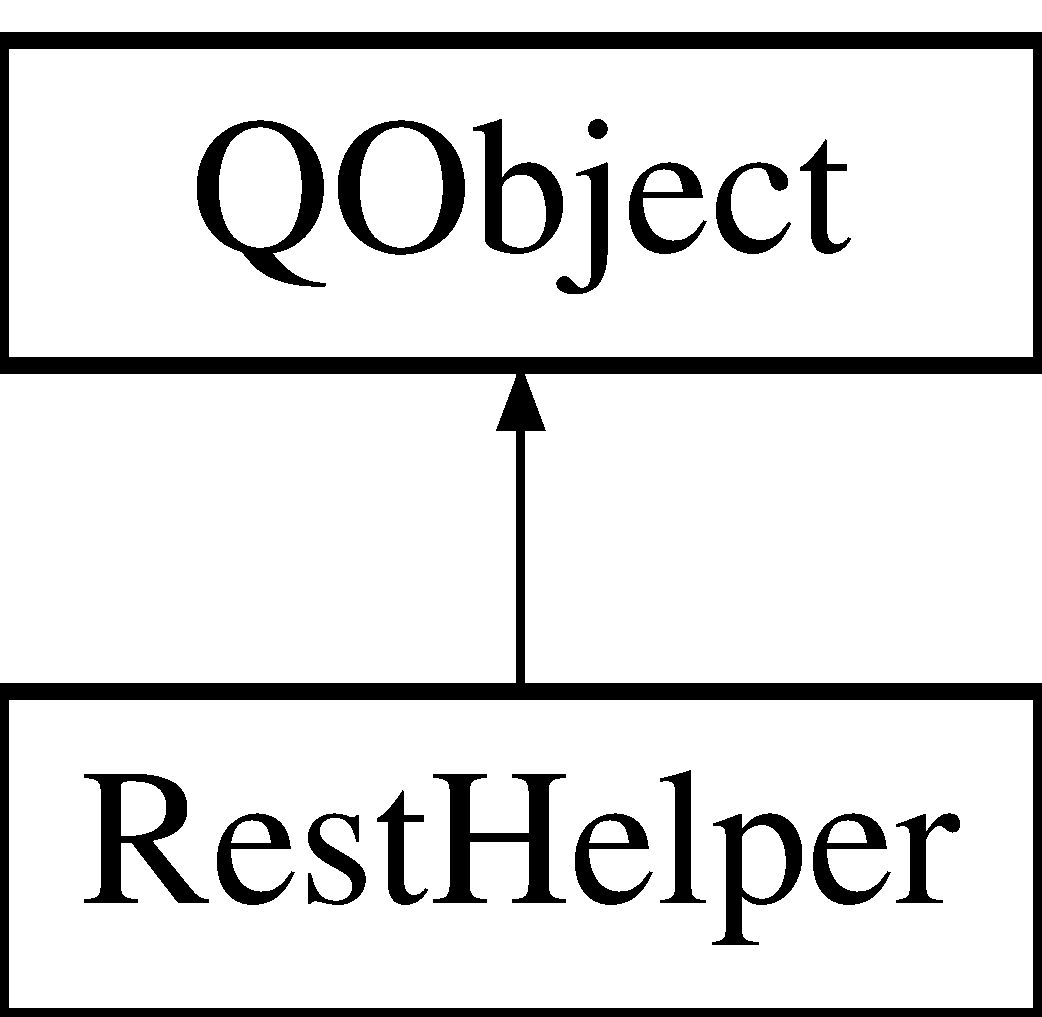
\includegraphics[height=2.000000cm]{class_rest_helper}
\end{center}
\end{figure}
\subsection*{Sloty publiczne}
\begin{DoxyCompactItemize}
\item 
\mbox{\Hypertarget{class_rest_helper_ae4960f651712c6ed66b032b3515b9f7b}\label{class_rest_helper_ae4960f651712c6ed66b032b3515b9f7b}} 
void \mbox{\hyperlink{class_rest_helper_ae4960f651712c6ed66b032b3515b9f7b}{fished}} ()
\begin{DoxyCompactList}\small\item\em fished Obsługuje zdarzenie zakończenia wysyłania danych \end{DoxyCompactList}\end{DoxyCompactItemize}
\subsection*{Metody publiczne}
\begin{DoxyCompactItemize}
\item 
\mbox{\Hypertarget{class_rest_helper_a52a1010ef31bfab8cafe7742c6206f71}\label{class_rest_helper_a52a1010ef31bfab8cafe7742c6206f71}} 
{\bfseries Rest\+Helper} (Q\+Object $\ast$parent=nullptr)
\item 
void \mbox{\hyperlink{class_rest_helper_ab27c5c6fdbe8f25c1b4a288a983f7995}{Send\+Color}} (Q\+Json\+Document json\+Doc, Q\+String api)
\begin{DoxyCompactList}\small\item\em Send\+Color Wysyła dokument J\+S\+ON do urządzenia. \end{DoxyCompactList}\item 
Q\+String \mbox{\hyperlink{class_rest_helper_ad6c71fc30c6377e10f465038b6b06c4c}{get\+Api\+Url}} ()
\begin{DoxyCompactList}\small\item\em get\+Api\+Url Zwraca adres IP urządzenia Raspberry\+Pi \end{DoxyCompactList}\item 
void \mbox{\hyperlink{class_rest_helper_ae0812d7e48940885625f939cf56b4072}{set\+Api\+Url}} (Q\+String url)
\begin{DoxyCompactList}\small\item\em set\+Api\+Url Modyfikuje adres IP urządzenia \end{DoxyCompactList}\item 
unsigned short \mbox{\hyperlink{class_rest_helper_ac4de88ea9cfe823ca317c87e99729b8c}{get\+Port}} ()
\begin{DoxyCompactList}\small\item\em get\+Port Zwraca port połączenia z urządzeniem \end{DoxyCompactList}\item 
void \mbox{\hyperlink{class_rest_helper_ac7748378a6d1dcfddf7dc5b803f9d4b2}{set\+Port}} (unsigned short port\+Num)
\begin{DoxyCompactList}\small\item\em set\+Port Modyfikuje wartość numeru portu połączenia \end{DoxyCompactList}\end{DoxyCompactItemize}
\subsection*{Statyczne metody publiczne}
\begin{DoxyCompactItemize}
\item 
static \mbox{\hyperlink{class_rest_helper}{Rest\+Helper}} \& \mbox{\hyperlink{class_rest_helper_aac5e384d8056c0d4a6398e83963fb2bf}{get\+Rest\+Helper}} ()
\begin{DoxyCompactList}\small\item\em get\+Rest\+Helper Zwraca referencję do istniejącego obiektu klasy lub, jeśli nie został wcześniej utworzony, inicjalizuje obiekt klasy \mbox{\hyperlink{class_rest_helper}{Rest\+Helper}} \end{DoxyCompactList}\end{DoxyCompactItemize}


\subsection{Opis szczegółowy}
The \mbox{\hyperlink{class_rest_helper}{Rest\+Helper}} class Klasa obsługuje wymianę danych pomiędzy aplikacją a A\+PI urządzenia Raspberry\+Pi. Klasa zgodna z wzorcem Singleton. 

\subsection{Dokumentacja funkcji składowych}
\mbox{\Hypertarget{class_rest_helper_ad6c71fc30c6377e10f465038b6b06c4c}\label{class_rest_helper_ad6c71fc30c6377e10f465038b6b06c4c}} 
\index{Rest\+Helper@{Rest\+Helper}!get\+Api\+Url@{get\+Api\+Url}}
\index{get\+Api\+Url@{get\+Api\+Url}!Rest\+Helper@{Rest\+Helper}}
\subsubsection{\texorpdfstring{get\+Api\+Url()}{getApiUrl()}}
{\footnotesize\ttfamily Q\+String Rest\+Helper\+::get\+Api\+Url (\begin{DoxyParamCaption}{ }\end{DoxyParamCaption})}



get\+Api\+Url Zwraca adres IP urządzenia Raspberry\+Pi 

\begin{DoxyReturn}{Zwraca}
Q\+String z adresem IP urządzenia 
\end{DoxyReturn}
\mbox{\Hypertarget{class_rest_helper_ac4de88ea9cfe823ca317c87e99729b8c}\label{class_rest_helper_ac4de88ea9cfe823ca317c87e99729b8c}} 
\index{Rest\+Helper@{Rest\+Helper}!get\+Port@{get\+Port}}
\index{get\+Port@{get\+Port}!Rest\+Helper@{Rest\+Helper}}
\subsubsection{\texorpdfstring{get\+Port()}{getPort()}}
{\footnotesize\ttfamily unsigned short Rest\+Helper\+::get\+Port (\begin{DoxyParamCaption}{ }\end{DoxyParamCaption})}



get\+Port Zwraca port połączenia z urządzeniem 

\begin{DoxyReturn}{Zwraca}
numer portu połączenia 
\end{DoxyReturn}
\mbox{\Hypertarget{class_rest_helper_aac5e384d8056c0d4a6398e83963fb2bf}\label{class_rest_helper_aac5e384d8056c0d4a6398e83963fb2bf}} 
\index{Rest\+Helper@{Rest\+Helper}!get\+Rest\+Helper@{get\+Rest\+Helper}}
\index{get\+Rest\+Helper@{get\+Rest\+Helper}!Rest\+Helper@{Rest\+Helper}}
\subsubsection{\texorpdfstring{get\+Rest\+Helper()}{getRestHelper()}}
{\footnotesize\ttfamily \mbox{\hyperlink{class_rest_helper}{Rest\+Helper}} \& Rest\+Helper\+::get\+Rest\+Helper (\begin{DoxyParamCaption}{ }\end{DoxyParamCaption})\hspace{0.3cm}{\ttfamily [static]}}



get\+Rest\+Helper Zwraca referencję do istniejącego obiektu klasy lub, jeśli nie został wcześniej utworzony, inicjalizuje obiekt klasy \mbox{\hyperlink{class_rest_helper}{Rest\+Helper}} 

\begin{DoxyReturn}{Zwraca}
referencja do obiektu klasy \mbox{\hyperlink{class_rest_helper}{Rest\+Helper}} 
\end{DoxyReturn}
\mbox{\Hypertarget{class_rest_helper_ab27c5c6fdbe8f25c1b4a288a983f7995}\label{class_rest_helper_ab27c5c6fdbe8f25c1b4a288a983f7995}} 
\index{Rest\+Helper@{Rest\+Helper}!Send\+Color@{Send\+Color}}
\index{Send\+Color@{Send\+Color}!Rest\+Helper@{Rest\+Helper}}
\subsubsection{\texorpdfstring{Send\+Color()}{SendColor()}}
{\footnotesize\ttfamily void Rest\+Helper\+::\+Send\+Color (\begin{DoxyParamCaption}\item[{Q\+Json\+Document}]{json\+Doc,  }\item[{Q\+String}]{api }\end{DoxyParamCaption})}



Send\+Color Wysyła dokument J\+S\+ON do urządzenia. 


\begin{DoxyParams}{Parametry}
{\em json\+Doc} & obiekt z danymi w notacji J\+S\+ON wysyłany do urządzenia \\
\hline
{\em api} & fragment adresu U\+RL do A\+PI urządzenia \\
\hline
\end{DoxyParams}
\mbox{\Hypertarget{class_rest_helper_ae0812d7e48940885625f939cf56b4072}\label{class_rest_helper_ae0812d7e48940885625f939cf56b4072}} 
\index{Rest\+Helper@{Rest\+Helper}!set\+Api\+Url@{set\+Api\+Url}}
\index{set\+Api\+Url@{set\+Api\+Url}!Rest\+Helper@{Rest\+Helper}}
\subsubsection{\texorpdfstring{set\+Api\+Url()}{setApiUrl()}}
{\footnotesize\ttfamily void Rest\+Helper\+::set\+Api\+Url (\begin{DoxyParamCaption}\item[{Q\+String}]{url }\end{DoxyParamCaption})}



set\+Api\+Url Modyfikuje adres IP urządzenia 


\begin{DoxyParams}{Parametry}
{\em url} & łańcuch znaków przypisywany polu api\+Url \\
\hline
\end{DoxyParams}
\mbox{\Hypertarget{class_rest_helper_ac7748378a6d1dcfddf7dc5b803f9d4b2}\label{class_rest_helper_ac7748378a6d1dcfddf7dc5b803f9d4b2}} 
\index{Rest\+Helper@{Rest\+Helper}!set\+Port@{set\+Port}}
\index{set\+Port@{set\+Port}!Rest\+Helper@{Rest\+Helper}}
\subsubsection{\texorpdfstring{set\+Port()}{setPort()}}
{\footnotesize\ttfamily void Rest\+Helper\+::set\+Port (\begin{DoxyParamCaption}\item[{unsigned short}]{port\+Num }\end{DoxyParamCaption})}



set\+Port Modyfikuje wartość numeru portu połączenia 


\begin{DoxyParams}{Parametry}
{\em port\+Num} & wartość przypisywana polu port \\
\hline
\end{DoxyParams}


Dokumentacja dla tej klasy została wygenerowana z plików\+:\begin{DoxyCompactItemize}
\item 
C\+:/\+Users/amy1/\+Source/\+Qt/\+Lampki\+App/\+Helpers/resthelper.\+h\item 
C\+:/\+Users/amy1/\+Source/\+Qt/\+Lampki\+App/\+Helpers/resthelper.\+cpp\end{DoxyCompactItemize}

\hypertarget{class_r_g_b_color_model}{}\section{Dokumentacja klasy R\+G\+B\+Color\+Model}
\label{class_r_g_b_color_model}\index{R\+G\+B\+Color\+Model@{R\+G\+B\+Color\+Model}}


The \mbox{\hyperlink{class_r_g_b_color_model}{R\+G\+B\+Color\+Model}} class Klasa dziedziczy po abstrakcyjnej klasie \mbox{\hyperlink{class_a_color_model}{A\+Color\+Model}}. Odpowiada za przetwarzanie danych dotyczacych koloru w przestrzeni barw R\+GB.  




{\ttfamily \#include $<$rgbcolormodel.\+h$>$}

Diagram dziedziczenia dla R\+G\+B\+Color\+Model\begin{figure}[H]
\begin{center}
\leavevmode
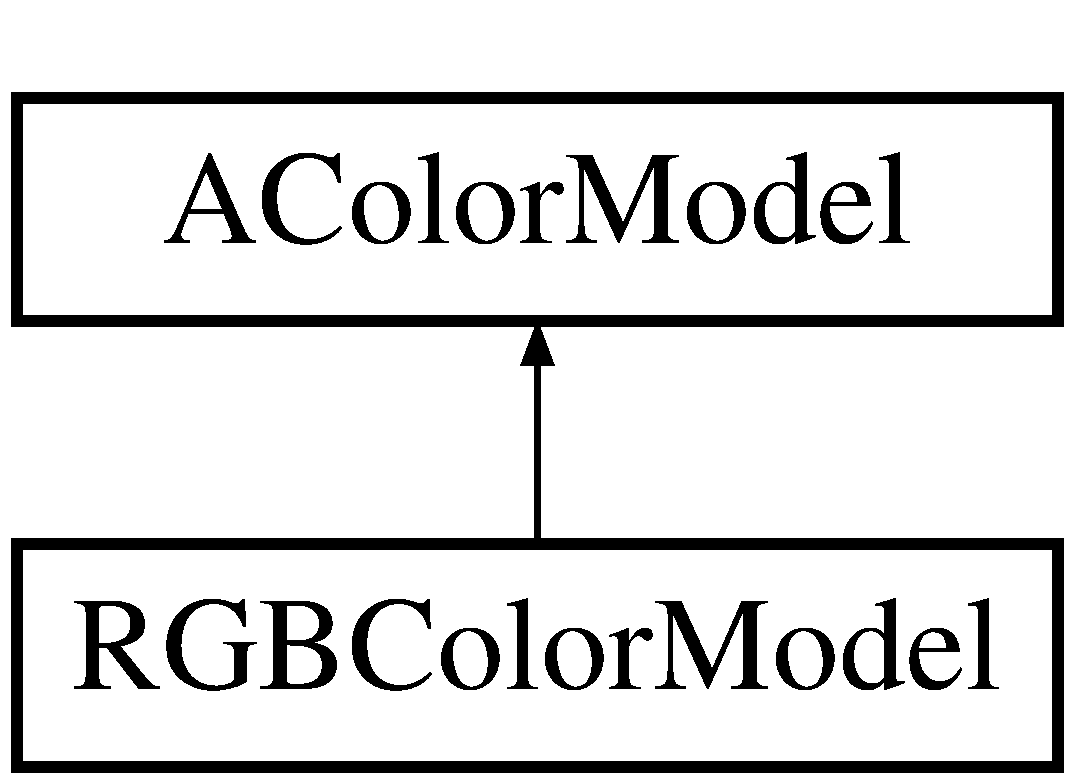
\includegraphics[height=2.000000cm]{class_r_g_b_color_model}
\end{center}
\end{figure}
\subsection*{Metody publiczne}
\begin{DoxyCompactItemize}
\item 
\mbox{\hyperlink{class_r_g_b_color_model_a60985479217d6c0f8dda2ec5d728a035}{R\+G\+B\+Color\+Model}} (int r, int g, int b)
\begin{DoxyCompactList}\small\item\em \mbox{\hyperlink{class_r_g_b_color_model}{R\+G\+B\+Color\+Model}} Inicjalizuje obiekt klasy \mbox{\hyperlink{class_r_g_b_color_model}{R\+G\+B\+Color\+Model}}. \end{DoxyCompactList}\item 
std\+::unique\+\_\+ptr$<$ \mbox{\hyperlink{class_a_color_model}{A\+Color\+Model}} $>$ \mbox{\hyperlink{class_r_g_b_color_model_a7619d529d6b0f94287221c813734244d}{As\+R\+GB}} () override
\begin{DoxyCompactList}\small\item\em As\+R\+GB Metoda przekazuje obiekt klasy \mbox{\hyperlink{class_r_g_b_color_model}{R\+G\+B\+Color\+Model}}. \end{DoxyCompactList}\item 
std\+::unique\+\_\+ptr$<$ \mbox{\hyperlink{class_a_color_model}{A\+Color\+Model}} $>$ \mbox{\hyperlink{class_r_g_b_color_model_a18d1b493d34f53ea4fdf9eaa066540c4}{As\+H\+SV}} () override
\begin{DoxyCompactList}\small\item\em As\+H\+SV Metoda wywołuje metodę parsującą Parse\+To\+H\+S\+V() i zwraca wynik konwersji. \end{DoxyCompactList}\item 
Q\+String \mbox{\hyperlink{class_r_g_b_color_model_ad1f82f637ab5b48c9e99b64270f38c54}{As\+Hex}} () override
\begin{DoxyCompactList}\small\item\em As\+Hex Konwertuje wartości składowe z systemu dziesiątkowego do systemu szesnastkowego przy pomocy String\+Stream, po czym łączy je w kod szesnastkowy koloru. \end{DoxyCompactList}\item 
int \mbox{\hyperlink{class_r_g_b_color_model_afd8f53b2cd42f3563db714978445a324}{Get\+RH}} () override
\begin{DoxyCompactList}\small\item\em Get\+RH. \end{DoxyCompactList}\item 
int \mbox{\hyperlink{class_r_g_b_color_model_ab90ddb80c57a81ca93b6c6b2aec21a88}{Get\+GS}} () override
\begin{DoxyCompactList}\small\item\em Get\+GS. \end{DoxyCompactList}\item 
int \mbox{\hyperlink{class_r_g_b_color_model_af87d29172cf3dc37e8b67926c323d521}{Get\+BV}} () override
\begin{DoxyCompactList}\small\item\em Get\+BV. \end{DoxyCompactList}\item 
void \mbox{\hyperlink{class_r_g_b_color_model_a2cfefda5444f0b9479aca4b661f1790b}{Set\+RH}} (int rh) override
\begin{DoxyCompactList}\small\item\em Set\+RH Modyfikuje wartość pola red. \end{DoxyCompactList}\item 
void \mbox{\hyperlink{class_r_g_b_color_model_a0b48f8097e7edf4a5e28e101a62c671a}{Set\+GS}} (int gs) override
\begin{DoxyCompactList}\small\item\em Set\+GS Modyfikuje wartość pola green. \end{DoxyCompactList}\item 
void \mbox{\hyperlink{class_r_g_b_color_model_ad3fa9841c0fa4082e06a81a3bbf57988}{Set\+BV}} (int bv) override
\begin{DoxyCompactList}\small\item\em Set\+BV Modyfikuje wartość pola blue. \end{DoxyCompactList}\end{DoxyCompactItemize}


\subsection{Opis szczegółowy}
The \mbox{\hyperlink{class_r_g_b_color_model}{R\+G\+B\+Color\+Model}} class Klasa dziedziczy po abstrakcyjnej klasie \mbox{\hyperlink{class_a_color_model}{A\+Color\+Model}}. Odpowiada za przetwarzanie danych dotyczacych koloru w przestrzeni barw R\+GB. 

\subsection{Dokumentacja konstruktora i destruktora}
\mbox{\Hypertarget{class_r_g_b_color_model_a60985479217d6c0f8dda2ec5d728a035}\label{class_r_g_b_color_model_a60985479217d6c0f8dda2ec5d728a035}} 
\index{R\+G\+B\+Color\+Model@{R\+G\+B\+Color\+Model}!R\+G\+B\+Color\+Model@{R\+G\+B\+Color\+Model}}
\index{R\+G\+B\+Color\+Model@{R\+G\+B\+Color\+Model}!R\+G\+B\+Color\+Model@{R\+G\+B\+Color\+Model}}
\subsubsection{\texorpdfstring{R\+G\+B\+Color\+Model()}{RGBColorModel()}}
{\footnotesize\ttfamily R\+G\+B\+Color\+Model\+::\+R\+G\+B\+Color\+Model (\begin{DoxyParamCaption}\item[{int}]{r,  }\item[{int}]{g,  }\item[{int}]{b }\end{DoxyParamCaption})}



\mbox{\hyperlink{class_r_g_b_color_model}{R\+G\+B\+Color\+Model}} Inicjalizuje obiekt klasy \mbox{\hyperlink{class_r_g_b_color_model}{R\+G\+B\+Color\+Model}}. 


\begin{DoxyParams}{Parametry}
{\em r} & Wartość do zainicjalizowania pola red \\
\hline
{\em g} & Wartość do zainicjalizowania pola green \\
\hline
{\em b} & Wartość do zainicjalizowania pola blue \\
\hline
\end{DoxyParams}


\subsection{Dokumentacja funkcji składowych}
\mbox{\Hypertarget{class_r_g_b_color_model_ad1f82f637ab5b48c9e99b64270f38c54}\label{class_r_g_b_color_model_ad1f82f637ab5b48c9e99b64270f38c54}} 
\index{R\+G\+B\+Color\+Model@{R\+G\+B\+Color\+Model}!As\+Hex@{As\+Hex}}
\index{As\+Hex@{As\+Hex}!R\+G\+B\+Color\+Model@{R\+G\+B\+Color\+Model}}
\subsubsection{\texorpdfstring{As\+Hex()}{AsHex()}}
{\footnotesize\ttfamily Q\+String R\+G\+B\+Color\+Model\+::\+As\+Hex (\begin{DoxyParamCaption}{ }\end{DoxyParamCaption})\hspace{0.3cm}{\ttfamily [override]}, {\ttfamily [virtual]}}



As\+Hex Konwertuje wartości składowe z systemu dziesiątkowego do systemu szesnastkowego przy pomocy String\+Stream, po czym łączy je w kod szesnastkowy koloru. 

\begin{DoxyReturn}{Zwraca}
Q\+String zawierający kod szesnastkowy koloru 
\end{DoxyReturn}


Implementuje \mbox{\hyperlink{class_a_color_model}{A\+Color\+Model}}.

\mbox{\Hypertarget{class_r_g_b_color_model_a18d1b493d34f53ea4fdf9eaa066540c4}\label{class_r_g_b_color_model_a18d1b493d34f53ea4fdf9eaa066540c4}} 
\index{R\+G\+B\+Color\+Model@{R\+G\+B\+Color\+Model}!As\+H\+SV@{As\+H\+SV}}
\index{As\+H\+SV@{As\+H\+SV}!R\+G\+B\+Color\+Model@{R\+G\+B\+Color\+Model}}
\subsubsection{\texorpdfstring{As\+H\+S\+V()}{AsHSV()}}
{\footnotesize\ttfamily std\+::unique\+\_\+ptr$<$ \mbox{\hyperlink{class_a_color_model}{A\+Color\+Model}} $>$ R\+G\+B\+Color\+Model\+::\+As\+H\+SV (\begin{DoxyParamCaption}{ }\end{DoxyParamCaption})\hspace{0.3cm}{\ttfamily [override]}, {\ttfamily [virtual]}}



As\+H\+SV Metoda wywołuje metodę parsującą Parse\+To\+H\+S\+V() i zwraca wynik konwersji. 

\begin{DoxyReturn}{Zwraca}
unique\+\_\+ptr do obiektu klasy \mbox{\hyperlink{class_h_s_v_color_model}{H\+S\+V\+Color\+Model}} 
\end{DoxyReturn}


Implementuje \mbox{\hyperlink{class_a_color_model}{A\+Color\+Model}}.

\mbox{\Hypertarget{class_r_g_b_color_model_a7619d529d6b0f94287221c813734244d}\label{class_r_g_b_color_model_a7619d529d6b0f94287221c813734244d}} 
\index{R\+G\+B\+Color\+Model@{R\+G\+B\+Color\+Model}!As\+R\+GB@{As\+R\+GB}}
\index{As\+R\+GB@{As\+R\+GB}!R\+G\+B\+Color\+Model@{R\+G\+B\+Color\+Model}}
\subsubsection{\texorpdfstring{As\+R\+G\+B()}{AsRGB()}}
{\footnotesize\ttfamily std\+::unique\+\_\+ptr$<$ \mbox{\hyperlink{class_a_color_model}{A\+Color\+Model}} $>$ R\+G\+B\+Color\+Model\+::\+As\+R\+GB (\begin{DoxyParamCaption}{ }\end{DoxyParamCaption})\hspace{0.3cm}{\ttfamily [override]}, {\ttfamily [virtual]}}



As\+R\+GB Metoda przekazuje obiekt klasy \mbox{\hyperlink{class_r_g_b_color_model}{R\+G\+B\+Color\+Model}}. 

\begin{DoxyReturn}{Zwraca}
unique\+\_\+ptr do obiektu klasy \mbox{\hyperlink{class_r_g_b_color_model}{R\+G\+B\+Color\+Model}} 
\end{DoxyReturn}


Implementuje \mbox{\hyperlink{class_a_color_model}{A\+Color\+Model}}.

\mbox{\Hypertarget{class_r_g_b_color_model_af87d29172cf3dc37e8b67926c323d521}\label{class_r_g_b_color_model_af87d29172cf3dc37e8b67926c323d521}} 
\index{R\+G\+B\+Color\+Model@{R\+G\+B\+Color\+Model}!Get\+BV@{Get\+BV}}
\index{Get\+BV@{Get\+BV}!R\+G\+B\+Color\+Model@{R\+G\+B\+Color\+Model}}
\subsubsection{\texorpdfstring{Get\+B\+V()}{GetBV()}}
{\footnotesize\ttfamily int R\+G\+B\+Color\+Model\+::\+Get\+BV (\begin{DoxyParamCaption}{ }\end{DoxyParamCaption})\hspace{0.3cm}{\ttfamily [override]}, {\ttfamily [virtual]}}



Get\+BV. 

\begin{DoxyReturn}{Zwraca}
wartość pola blue 
\end{DoxyReturn}


Implementuje \mbox{\hyperlink{class_a_color_model}{A\+Color\+Model}}.

\mbox{\Hypertarget{class_r_g_b_color_model_ab90ddb80c57a81ca93b6c6b2aec21a88}\label{class_r_g_b_color_model_ab90ddb80c57a81ca93b6c6b2aec21a88}} 
\index{R\+G\+B\+Color\+Model@{R\+G\+B\+Color\+Model}!Get\+GS@{Get\+GS}}
\index{Get\+GS@{Get\+GS}!R\+G\+B\+Color\+Model@{R\+G\+B\+Color\+Model}}
\subsubsection{\texorpdfstring{Get\+G\+S()}{GetGS()}}
{\footnotesize\ttfamily int R\+G\+B\+Color\+Model\+::\+Get\+GS (\begin{DoxyParamCaption}{ }\end{DoxyParamCaption})\hspace{0.3cm}{\ttfamily [override]}, {\ttfamily [virtual]}}



Get\+GS. 

\begin{DoxyReturn}{Zwraca}
wartość pola green 
\end{DoxyReturn}


Implementuje \mbox{\hyperlink{class_a_color_model}{A\+Color\+Model}}.

\mbox{\Hypertarget{class_r_g_b_color_model_afd8f53b2cd42f3563db714978445a324}\label{class_r_g_b_color_model_afd8f53b2cd42f3563db714978445a324}} 
\index{R\+G\+B\+Color\+Model@{R\+G\+B\+Color\+Model}!Get\+RH@{Get\+RH}}
\index{Get\+RH@{Get\+RH}!R\+G\+B\+Color\+Model@{R\+G\+B\+Color\+Model}}
\subsubsection{\texorpdfstring{Get\+R\+H()}{GetRH()}}
{\footnotesize\ttfamily int R\+G\+B\+Color\+Model\+::\+Get\+RH (\begin{DoxyParamCaption}{ }\end{DoxyParamCaption})\hspace{0.3cm}{\ttfamily [override]}, {\ttfamily [virtual]}}



Get\+RH. 

\begin{DoxyReturn}{Zwraca}
wartość pola red 
\end{DoxyReturn}


Implementuje \mbox{\hyperlink{class_a_color_model}{A\+Color\+Model}}.

\mbox{\Hypertarget{class_r_g_b_color_model_ad3fa9841c0fa4082e06a81a3bbf57988}\label{class_r_g_b_color_model_ad3fa9841c0fa4082e06a81a3bbf57988}} 
\index{R\+G\+B\+Color\+Model@{R\+G\+B\+Color\+Model}!Set\+BV@{Set\+BV}}
\index{Set\+BV@{Set\+BV}!R\+G\+B\+Color\+Model@{R\+G\+B\+Color\+Model}}
\subsubsection{\texorpdfstring{Set\+B\+V()}{SetBV()}}
{\footnotesize\ttfamily void R\+G\+B\+Color\+Model\+::\+Set\+BV (\begin{DoxyParamCaption}\item[{int}]{bv }\end{DoxyParamCaption})\hspace{0.3cm}{\ttfamily [override]}, {\ttfamily [virtual]}}



Set\+BV Modyfikuje wartość pola blue. 


\begin{DoxyParams}{Parametry}
{\em bv} & Wartość przypisywana składowej blue \\
\hline
\end{DoxyParams}


Implementuje \mbox{\hyperlink{class_a_color_model}{A\+Color\+Model}}.

\mbox{\Hypertarget{class_r_g_b_color_model_a0b48f8097e7edf4a5e28e101a62c671a}\label{class_r_g_b_color_model_a0b48f8097e7edf4a5e28e101a62c671a}} 
\index{R\+G\+B\+Color\+Model@{R\+G\+B\+Color\+Model}!Set\+GS@{Set\+GS}}
\index{Set\+GS@{Set\+GS}!R\+G\+B\+Color\+Model@{R\+G\+B\+Color\+Model}}
\subsubsection{\texorpdfstring{Set\+G\+S()}{SetGS()}}
{\footnotesize\ttfamily void R\+G\+B\+Color\+Model\+::\+Set\+GS (\begin{DoxyParamCaption}\item[{int}]{gs }\end{DoxyParamCaption})\hspace{0.3cm}{\ttfamily [override]}, {\ttfamily [virtual]}}



Set\+GS Modyfikuje wartość pola green. 


\begin{DoxyParams}{Parametry}
{\em gs} & Wartość przypisywana składowej green \\
\hline
\end{DoxyParams}


Implementuje \mbox{\hyperlink{class_a_color_model}{A\+Color\+Model}}.

\mbox{\Hypertarget{class_r_g_b_color_model_a2cfefda5444f0b9479aca4b661f1790b}\label{class_r_g_b_color_model_a2cfefda5444f0b9479aca4b661f1790b}} 
\index{R\+G\+B\+Color\+Model@{R\+G\+B\+Color\+Model}!Set\+RH@{Set\+RH}}
\index{Set\+RH@{Set\+RH}!R\+G\+B\+Color\+Model@{R\+G\+B\+Color\+Model}}
\subsubsection{\texorpdfstring{Set\+R\+H()}{SetRH()}}
{\footnotesize\ttfamily void R\+G\+B\+Color\+Model\+::\+Set\+RH (\begin{DoxyParamCaption}\item[{int}]{rh }\end{DoxyParamCaption})\hspace{0.3cm}{\ttfamily [override]}, {\ttfamily [virtual]}}



Set\+RH Modyfikuje wartość pola red. 


\begin{DoxyParams}{Parametry}
{\em rh} & Wartość przypisywana składowej red \\
\hline
\end{DoxyParams}


Implementuje \mbox{\hyperlink{class_a_color_model}{A\+Color\+Model}}.



Dokumentacja dla tej klasy została wygenerowana z plików\+:\begin{DoxyCompactItemize}
\item 
C\+:/\+Users/amy1/\+Source/\+Qt/\+Lampki\+App/\+Models/rgbcolormodel.\+h\item 
C\+:/\+Users/amy1/\+Source/\+Qt/\+Lampki\+App/\+Models/rgbcolormodel.\+cpp\end{DoxyCompactItemize}

\hypertarget{classsettings_view_model}{}\section{Dokumentacja klasy settings\+View\+Model}
\label{classsettings_view_model}\index{settings\+View\+Model@{settings\+View\+Model}}


The \mbox{\hyperlink{classsettings_view_model}{settings\+View\+Model}} class Klasa obsługuje komunikację między Rest\+Helperem a UI -\/ pozwala na modyfikację przez użytkownika ustawień połączenia z urządzeniem Raspberry PI.  




{\ttfamily \#include $<$settingsviewmodel.\+h$>$}

Diagram dziedziczenia dla settings\+View\+Model\begin{figure}[H]
\begin{center}
\leavevmode
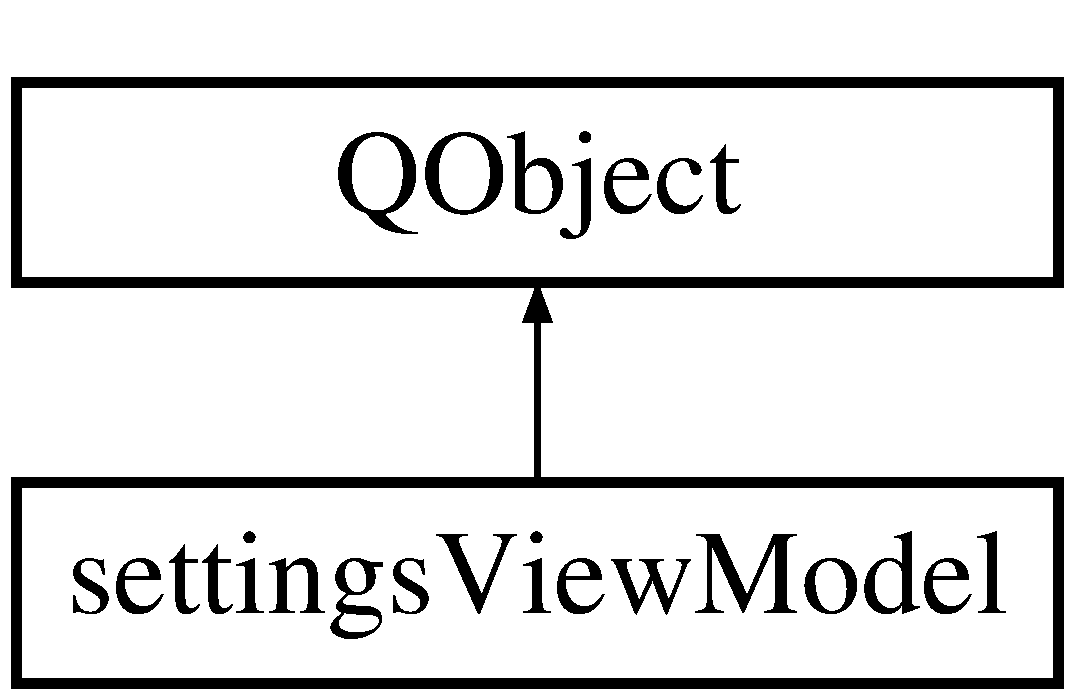
\includegraphics[height=2.000000cm]{classsettings_view_model}
\end{center}
\end{figure}
\subsection*{Sloty publiczne}
\begin{DoxyCompactItemize}
\item 
void \mbox{\hyperlink{classsettings_view_model_a2ffae7dd1ad8acfa8179366bdba7ec19}{set\+Url}} (Q\+String url\+Str)
\begin{DoxyCompactList}\small\item\em set\+Url Modyfikuje właściwość Url \end{DoxyCompactList}\item 
void \mbox{\hyperlink{classsettings_view_model_a893273de2f0be7d15d2c1e17ded4be0c}{set\+Port}} (unsigned short port\+Num)
\begin{DoxyCompactList}\small\item\em set\+Port Modyfikuje właściwość Port \end{DoxyCompactList}\end{DoxyCompactItemize}
\subsection*{Sygnały}
\begin{DoxyCompactItemize}
\item 
void \mbox{\hyperlink{classsettings_view_model_a7e9a10f475bc4b11ec576cf527070d10}{url\+Changed}} (Q\+String arg)
\begin{DoxyCompactList}\small\item\em url\+Changed Informuje o zmianie adresu IP przez użytkownika \end{DoxyCompactList}\item 
void \mbox{\hyperlink{classsettings_view_model_ab0cf0ae85d3173dea74ed54dae9fef73}{port\+Changed}} (unsigned short arg)
\begin{DoxyCompactList}\small\item\em port\+Changed Informuje o zmianie portu przez użytkownika \end{DoxyCompactList}\end{DoxyCompactItemize}
\subsection*{Metody publiczne}
\begin{DoxyCompactItemize}
\item 
\mbox{\Hypertarget{classsettings_view_model_ac5d71573c7aefd1a2ba0f4486a351038}\label{classsettings_view_model_ac5d71573c7aefd1a2ba0f4486a351038}} 
{\bfseries settings\+View\+Model} (Q\+Object $\ast$parent=nullptr)
\item 
Q\+String \mbox{\hyperlink{classsettings_view_model_a6f81d1950b115d808899e5ea2fa607b3}{get\+Url}} ()
\begin{DoxyCompactList}\small\item\em get\+Url \end{DoxyCompactList}\item 
unsigned short \mbox{\hyperlink{classsettings_view_model_a021d67fc746244e4522cc6f38656cc1d}{get\+Port}} ()
\begin{DoxyCompactList}\small\item\em get\+Port \end{DoxyCompactList}\item 
\mbox{\Hypertarget{classsettings_view_model_ab8a556ced5fbba706bbc876865b242ad}\label{classsettings_view_model_ab8a556ced5fbba706bbc876865b242ad}} 
Q\+\_\+\+I\+N\+V\+O\+K\+A\+B\+LE Q\+String {\bfseries get\+Url\+From\+Settings} ()
\item 
\mbox{\Hypertarget{classsettings_view_model_a42a859605ffdc083f5a9e906c4951ab0}\label{classsettings_view_model_a42a859605ffdc083f5a9e906c4951ab0}} 
Q\+\_\+\+I\+N\+V\+O\+K\+A\+B\+LE unsigned short {\bfseries get\+Port\+From\+Settings} ()
\item 
\mbox{\Hypertarget{classsettings_view_model_ab53dce825dff35b4bbd9e65a60c1b7b0}\label{classsettings_view_model_ab53dce825dff35b4bbd9e65a60c1b7b0}} 
Q\+\_\+\+I\+N\+V\+O\+K\+A\+B\+LE void {\bfseries set\+Settings} ()
\end{DoxyCompactItemize}
\subsection*{Właściwości}
\begin{DoxyCompactItemize}
\item 
\mbox{\Hypertarget{classsettings_view_model_af82b4874e05dd9dba5dde4cf46f8d94d}\label{classsettings_view_model_af82b4874e05dd9dba5dde4cf46f8d94d}} 
Q\+String {\bfseries Url}
\item 
\mbox{\Hypertarget{classsettings_view_model_ac352510bc5895c88437107b000988935}\label{classsettings_view_model_ac352510bc5895c88437107b000988935}} 
unsigned short Port {\bfseries R\+E\+AD}
\end{DoxyCompactItemize}


\subsection{Opis szczegółowy}
The \mbox{\hyperlink{classsettings_view_model}{settings\+View\+Model}} class Klasa obsługuje komunikację między Rest\+Helperem a UI -\/ pozwala na modyfikację przez użytkownika ustawień połączenia z urządzeniem Raspberry PI. 

\subsection{Dokumentacja funkcji składowych}
\mbox{\Hypertarget{classsettings_view_model_a021d67fc746244e4522cc6f38656cc1d}\label{classsettings_view_model_a021d67fc746244e4522cc6f38656cc1d}} 
\index{settings\+View\+Model@{settings\+View\+Model}!get\+Port@{get\+Port}}
\index{get\+Port@{get\+Port}!settings\+View\+Model@{settings\+View\+Model}}
\subsubsection{\texorpdfstring{get\+Port()}{getPort()}}
{\footnotesize\ttfamily unsigned short settings\+View\+Model\+::get\+Port (\begin{DoxyParamCaption}{ }\end{DoxyParamCaption})}



get\+Port 

\begin{DoxyReturn}{Zwraca}
Zwraca port połączenia w formie wartości numerycznej 
\end{DoxyReturn}
\mbox{\Hypertarget{classsettings_view_model_a6f81d1950b115d808899e5ea2fa607b3}\label{classsettings_view_model_a6f81d1950b115d808899e5ea2fa607b3}} 
\index{settings\+View\+Model@{settings\+View\+Model}!get\+Url@{get\+Url}}
\index{get\+Url@{get\+Url}!settings\+View\+Model@{settings\+View\+Model}}
\subsubsection{\texorpdfstring{get\+Url()}{getUrl()}}
{\footnotesize\ttfamily Q\+String settings\+View\+Model\+::get\+Url (\begin{DoxyParamCaption}{ }\end{DoxyParamCaption})}



get\+Url 

\begin{DoxyReturn}{Zwraca}
Zwraca adres IP urządzenia w formie łańcucha znaków 
\end{DoxyReturn}
\mbox{\Hypertarget{classsettings_view_model_ab0cf0ae85d3173dea74ed54dae9fef73}\label{classsettings_view_model_ab0cf0ae85d3173dea74ed54dae9fef73}} 
\index{settings\+View\+Model@{settings\+View\+Model}!port\+Changed@{port\+Changed}}
\index{port\+Changed@{port\+Changed}!settings\+View\+Model@{settings\+View\+Model}}
\subsubsection{\texorpdfstring{port\+Changed}{portChanged}}
{\footnotesize\ttfamily void settings\+View\+Model\+::port\+Changed (\begin{DoxyParamCaption}\item[{unsigned short}]{arg }\end{DoxyParamCaption})\hspace{0.3cm}{\ttfamily [signal]}}



port\+Changed Informuje o zmianie portu przez użytkownika 


\begin{DoxyParams}{Parametry}
{\em arg} & numeryczna wartość numeru portu \\
\hline
\end{DoxyParams}
\mbox{\Hypertarget{classsettings_view_model_a893273de2f0be7d15d2c1e17ded4be0c}\label{classsettings_view_model_a893273de2f0be7d15d2c1e17ded4be0c}} 
\index{settings\+View\+Model@{settings\+View\+Model}!set\+Port@{set\+Port}}
\index{set\+Port@{set\+Port}!settings\+View\+Model@{settings\+View\+Model}}
\subsubsection{\texorpdfstring{set\+Port}{setPort}}
{\footnotesize\ttfamily void settings\+View\+Model\+::set\+Port (\begin{DoxyParamCaption}\item[{unsigned short}]{port\+Num }\end{DoxyParamCaption})\hspace{0.3cm}{\ttfamily [slot]}}



set\+Port Modyfikuje właściwość Port 


\begin{DoxyParams}{Parametry}
{\em port\+Num} & wpisany numer portu \\
\hline
\end{DoxyParams}
\mbox{\Hypertarget{classsettings_view_model_a2ffae7dd1ad8acfa8179366bdba7ec19}\label{classsettings_view_model_a2ffae7dd1ad8acfa8179366bdba7ec19}} 
\index{settings\+View\+Model@{settings\+View\+Model}!set\+Url@{set\+Url}}
\index{set\+Url@{set\+Url}!settings\+View\+Model@{settings\+View\+Model}}
\subsubsection{\texorpdfstring{set\+Url}{setUrl}}
{\footnotesize\ttfamily void settings\+View\+Model\+::set\+Url (\begin{DoxyParamCaption}\item[{Q\+String}]{url\+Str }\end{DoxyParamCaption})\hspace{0.3cm}{\ttfamily [slot]}}



set\+Url Modyfikuje właściwość Url 


\begin{DoxyParams}{Parametry}
{\em url\+Str} & wpisany adres IP \\
\hline
\end{DoxyParams}
\mbox{\Hypertarget{classsettings_view_model_a7e9a10f475bc4b11ec576cf527070d10}\label{classsettings_view_model_a7e9a10f475bc4b11ec576cf527070d10}} 
\index{settings\+View\+Model@{settings\+View\+Model}!url\+Changed@{url\+Changed}}
\index{url\+Changed@{url\+Changed}!settings\+View\+Model@{settings\+View\+Model}}
\subsubsection{\texorpdfstring{url\+Changed}{urlChanged}}
{\footnotesize\ttfamily void settings\+View\+Model\+::url\+Changed (\begin{DoxyParamCaption}\item[{Q\+String}]{arg }\end{DoxyParamCaption})\hspace{0.3cm}{\ttfamily [signal]}}



url\+Changed Informuje o zmianie adresu IP przez użytkownika 


\begin{DoxyParams}{Parametry}
{\em arg} & wpisany przez użytkownika adres IP \\
\hline
\end{DoxyParams}


Dokumentacja dla tej klasy została wygenerowana z plików\+:\begin{DoxyCompactItemize}
\item 
C\+:/\+Users/amy1/\+Source/\+Qt/\+Lampki\+App/\+View\+Models/settingsviewmodel.\+h\item 
C\+:/\+Users/amy1/\+Source/\+Qt/\+Lampki\+App/\+View\+Models/settingsviewmodel.\+cpp\end{DoxyCompactItemize}

%--- End generated contents ---

% Index
\backmatter
\newpage
\phantomsection
\clearemptydoublepage
\addcontentsline{toc}{chapter}{Indeks}
\printindex

\end{document}
